%%%%%%%%%%%%%%%%%%%%%%%%%%%%%%%%%%%%%%%%%%  不使用 authblk 包制作标题  %%%%%%%%%%%%%%%%%%%%%%%%%%%%%%%%%%%%%%%%%%%%%%
%-------------------------------PPT Title-------------------------------------
\title{AI~For~Science:~\\知识图谱和大模型\\在化学-化工领域的实现}
%-----------------------------------------------------------------------------

%----------------------------Author & Date------------------------------------
%\author[\textrm{Jun\_Jiang}]{姜\;\;骏\inst{}} %[]{} (optional, use only with lots of authors)
%% - Give the names in the same order as the appear in the paper.
%% - Use the \inst{?} command only if the authors have different
%%   affiliation.
\institute[BCC]{\inst{}%
%\institute[Gain~Strong]{\inst{}%
\vskip 2pt 中科合成油技术有限公司\\
\vskip 3pt 北京市计算中心}
%云平台事业部~材料计算团队}
%\vskip -20pt {\large 格致斯创~科技}}
\date[\today] % (optional, should be abbreviation of conference name)
{	%{\fontsize{6.2pt}{4.2pt}\selectfont{\textcolor{blue}{E-mail:~}\url{jiangjun@bcc.ac.cn}}}
\vskip 15 pt {\fontsize{8.2pt}{6.2pt}\selectfont{%清华大学\;\;物理系% 报告地点
	\vskip 5 pt \textrm{2024.07.12}}}
}

%% - Either use conference name or its abbreviation
%% - Not really information to the audience, more for people (including
%%   yourself) who are reading the slides onlin%%   yourself) who are reading the slides onlin%%   yourself) who are reading the slides onlineee
%%%%%%%%%%%%%%%%%%%%%%%%%%%%%%%%%%%%%%%%%%%%%%%%%%%%%%%%%%%%%%%%%%%%%%%%%%%%%%%%%%%%%%%%%%%%%%%%%%%%%%%%%%%%%%%%%%%%%

\subject{}
% This is only inserted into the PDF information catalog. Can be left
% out.
%\maketitle
\frame
{
%	\frametitle{\fontsize{9.5pt}{5.2pt}\selectfont{\textcolor{orange}{“大数据中心调研座谈会”}}}
\titlepage
}
%-----------------------------------------------------------------------------

%------------------------------------------------------------------------------列出全文 outline ---------------------------------------------------------------------------------
\section*{}
\frame[allowframebreaks]
{
  \frametitle{Outline}
%  \frametitle{\textcolor{mycolor}{\secname}}
  \tableofcontents%[current,currentsection,currentsubsection]
}
%在每个section之前列出全部Outline
%类似的在每个subsection之前列出全部Outline是\AtBeginSubsection[]
%\AtBeginSection[]
%{
%  \frame<handout:0>%[allowframebreaks]
%  {
%    \frametitle{Outline}
%%全部Outline中,本部分加亮
%    \tableofcontents[current,currentsection]
%  }
%}

%-----------------------------------------------PPT main Body------------------------------------------------------------------------------------
\small
\begin{frame}{科学研究的重要助手:~计算模拟}
\begin{figure}[h!]
\vspace*{-0.18in}
\centering
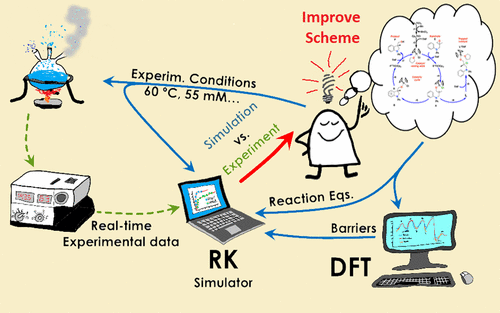
\includegraphics[height=2.55in,width=4.05in]{Figures/Schematic_Material-Design.png}
%\caption{\tiny \textrm{Pseudopotential for metallic sodium, based on the empty core model and screened by the Thomas-Fermi dielectric function.}}%(与文献\cite{EPJB33-47_2003}图1对比)
%\caption{\tiny \textrm{Pseudopotential for metallic sodium, based on the empty core model and screened by the Thomas-Fermi dielectric function.}}%(与文献\cite{EPJB33-47_2003}图1对比)
\label{Schematic_Material-Design}
\end{figure}
\end{frame}

\frame
{
	\frametitle{材料模拟的基本思想和方法}
\begin{figure}[h!]
\vspace*{-0.25in}
\centering
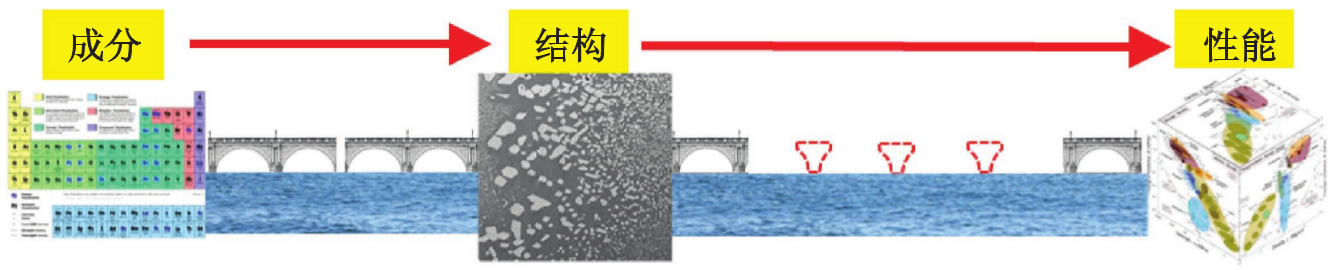
\includegraphics[height=0.80in,width=4.05in]{Figures/MGE-2.png}
%\caption{\tiny \textrm{Pseudopotential for metallic sodium, based on the empty core model and screened by the Thomas-Fermi dielectric function.}}%(与文献\cite{EPJB33-47_2003}图1对比)
\label{MGE}
\end{figure}
\begin{minipage}[c]{0.30\textwidth}
\begin{itemize}%[+-| alert@+>]
\vspace*{-2.25in}
 {\fontsize{7.5pt}{6.0pt}\selectfont
	 \setlength{\itemsep}{10pt}
 \item 变革研发模式,计算-实验-理论-数据科学相融合: 高效、低耗按需设计
 \item 数据驱动的材料创新平台主要面向复杂材料的模拟}
 \end{itemize}
\end{minipage}
\hfill
\begin{minipage}[b]{0.68\textwidth}
\begin{figure}[h!]
%\vspace*{-0.25in}
\centering
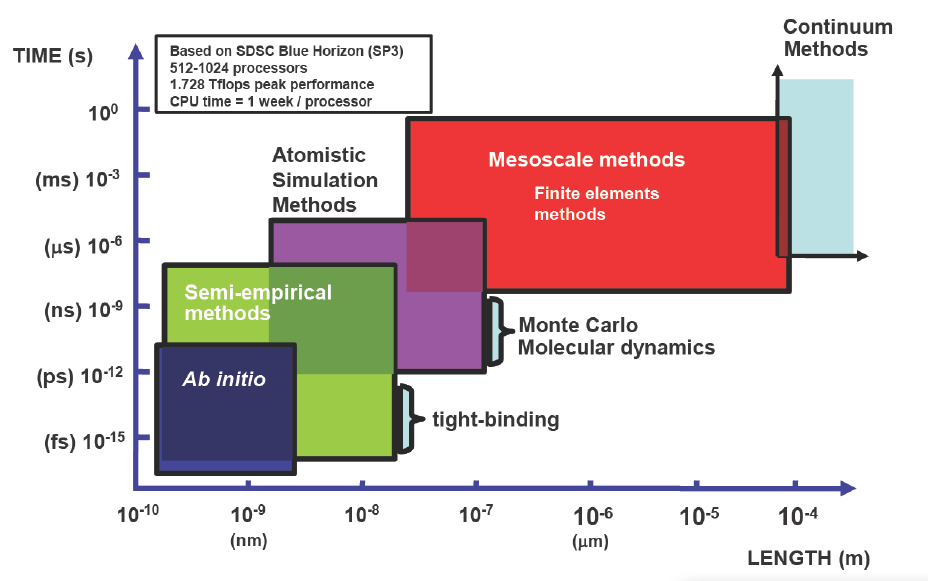
\includegraphics[height=1.80in,width=2.75in]{Figures/Multi-Scale-6.png}
%\caption{\tiny \textrm{Pseudopotential for metallic sodium, based on the empty core model and screened by the Thomas-Fermi dielectric function.}}%(与文献\cite{EPJB33-47_2003}图1对比)
\label{Multi-Scale}
\end{figure}
\end{minipage}
}

\frame
{
	\frametitle{科学研究的范式变更}
\begin{figure}[h!]
\vspace*{-0.28in}
\centering
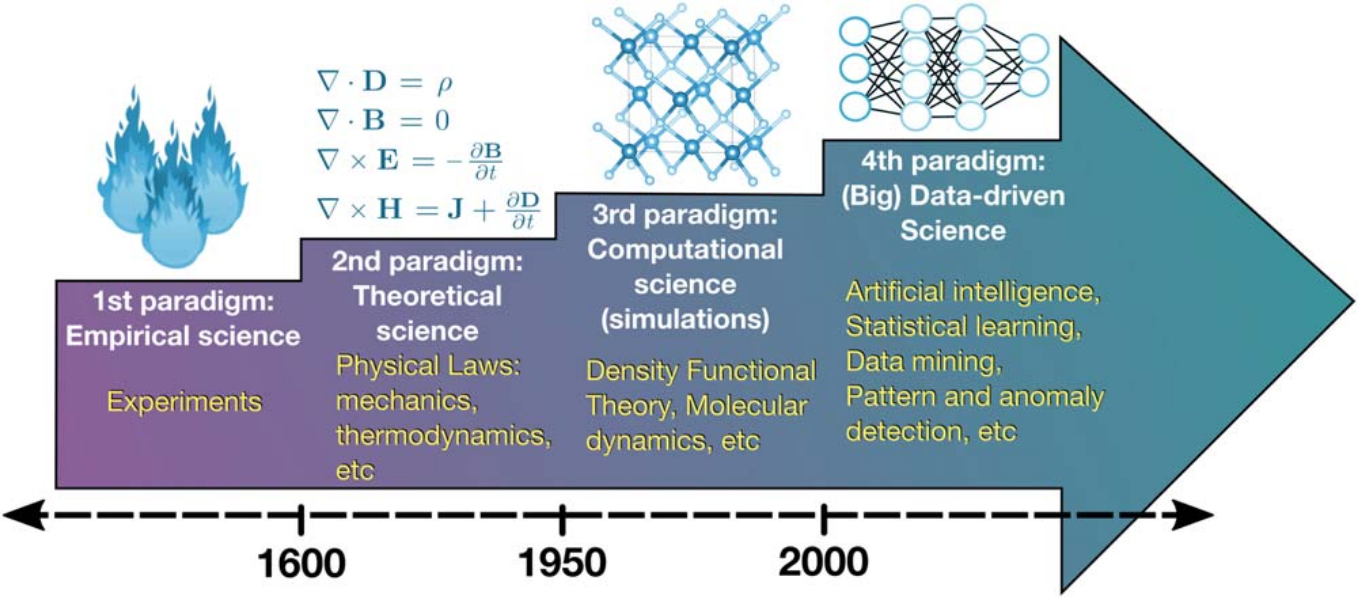
\includegraphics[height=2.00in,width=4.15in]{Figures/Four_Model_3.png}
%\caption{\tiny \textrm{Pseudopotential for metallic sodium, based on the empty core model and screened by the Thomas-Fermi dielectric function.}}%(与文献\cite{EPJB33-47_2003}图1对比)
\label{Four_Model}
\end{figure}
\begin{minipage}[b]{0.48\textwidth}
 {\fontsize{7.5pt}{6.0pt}\selectfont\begin{itemize}%[+-| alert@+>]
	 \setlength{\itemsep}{10pt}
 \item 逐步趋于理性
 \item 逐步趋于复杂
 \end{itemize}}
\end{minipage}
\hfill
\begin{minipage}[b]{0.48\textwidth}
 {\fontsize{7.5pt}{6.0pt}\selectfont\begin{itemize}%[+-| alert@+>]
	 \setlength{\itemsep}{10pt}
 \item 逐步趋于抽象
 \item 逐步趋于深刻
 \end{itemize}}
\end{minipage}
}

\frame
{
	\frametitle{数据驱动的科学研究}
前所未有的计算能力和大规模的数据收集能力%,现代科学正在进入“第四范式”:
\begin{figure}[h!]
%\vspace*{-0.05in}
\centering
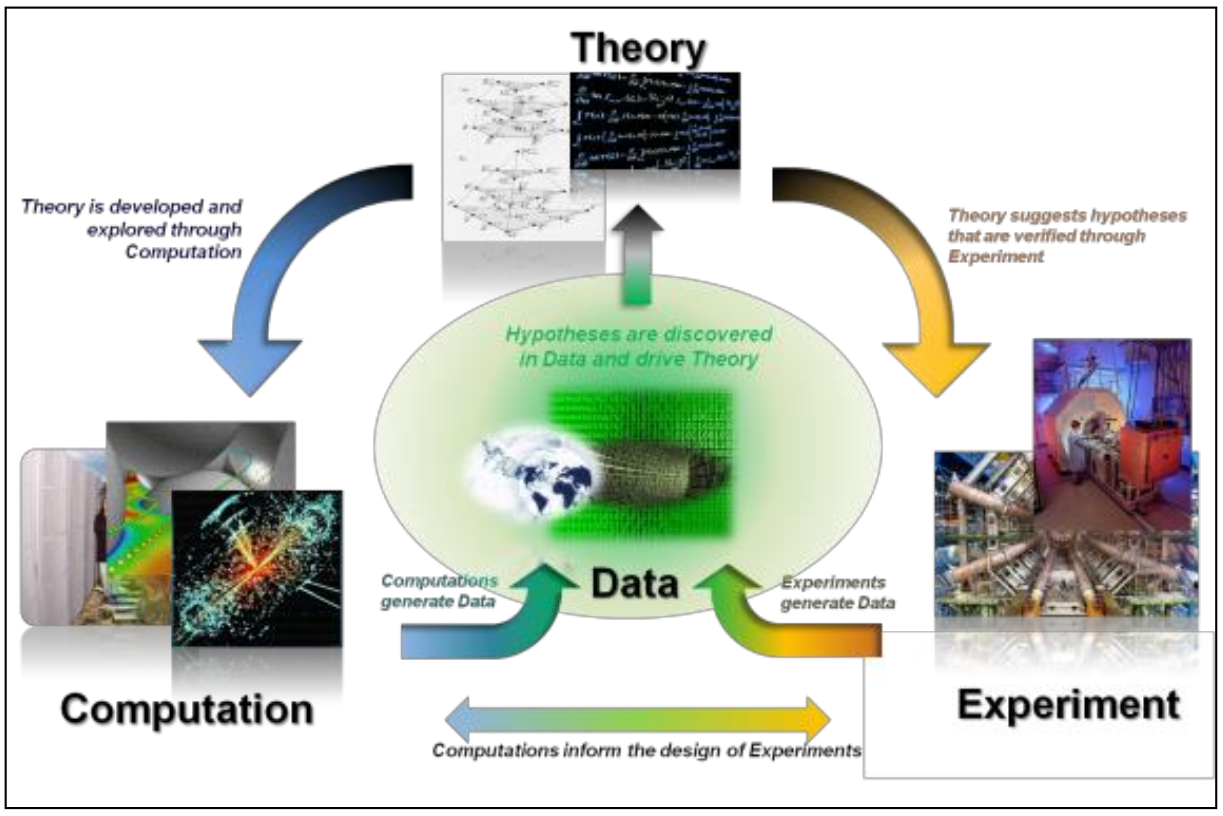
\includegraphics[height=2.30in,width=3.70in]{Figures/Four_Model_1.png}
%\caption{\tiny \textrm{Pseudopotential for metallic sodium, based on the empty core model and screened by the Thomas-Fermi dielectric function.}}%(与文献\cite{EPJB33-47_2003}图1对比)
\label{Four_Model_1}
\end{figure}
科学的新驱动力:~\textcolor{red}{密集数据}+\textcolor{red}{人工智能}\\
}

\frame
{
	\frametitle{数据、信息与知识}
\begin{figure}[h!]
\centering
\vskip -10pt
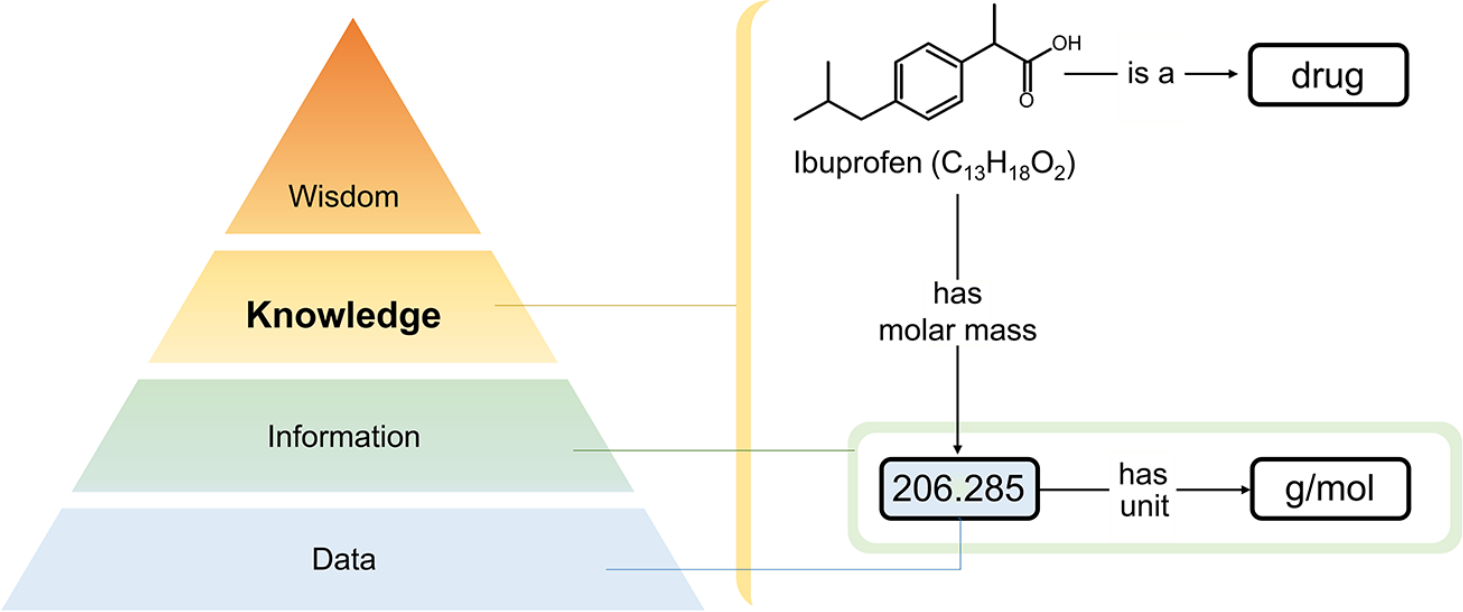
\includegraphics[height=1.75in,width=4.00in,viewport=0 0 1490 615,clip]{Figures/DIKW_pyramid-illustrating-data_information-knowledge.png}
\caption{\tiny\textrm{Schematic representation of the DIKW pyramid illustrating the meaning of data, inforamation, and knowledge in the chemical context.\cite{ACR56-128_2023}}}%(与文献\cite{EPJB33-47_2003}图1对比)
\label{Fig:Knowledge-based_system}
\end{figure}
\textcolor{magenta}{知识}\textrm{(Knowledge)}:\\
哲学学科——诸如认知论和方法论——中的核心主题
}

\begin{frame}
	\frametitle{化学-化工知识组织的技术实现}
	以知识图谱为例,说明(煤)化学-化工类知识采集、分类与组织
\begin{figure}[h!]
%\vspace*{-0.05in}
\centering
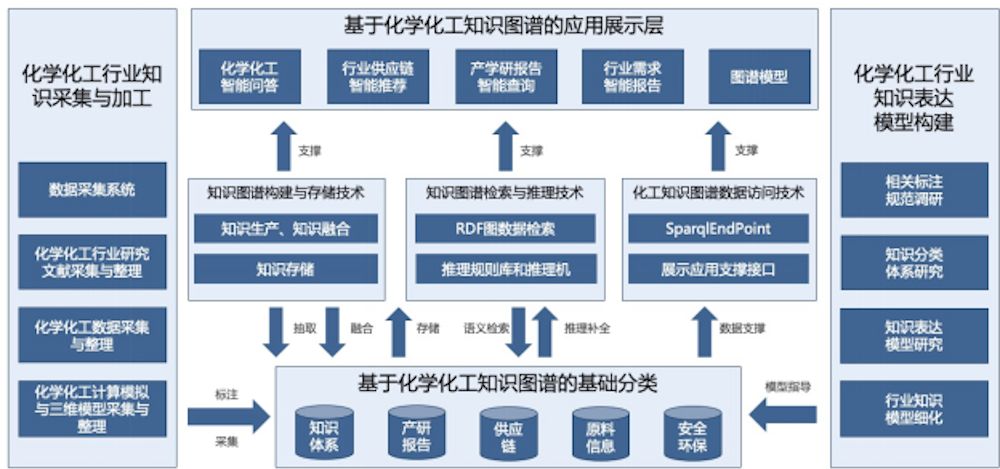
\includegraphics[height=2.08in,width=4.00in,viewport=0 0 245 113,clip]{Figures/KG_Chem-Frame.png}
\caption{\tiny 项目总体技术框架.}%(与文献\cite{EPJB33-47_2003}图1对比)
\label{KG_Chem-Frame}
\end{figure}
\end{frame}

\begin{frame}
	\frametitle{化学-化工知识的数据采集}
\begin{figure}[h!]
%\vspace*{-0.05in}
\centering
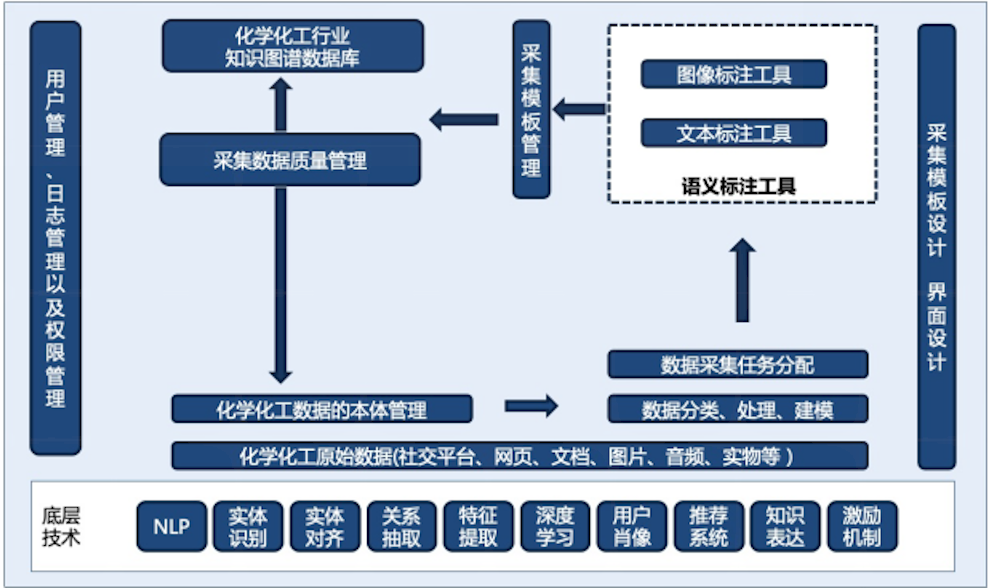
\includegraphics[height=2.30in,width=4.00in,viewport=0 0 240 150,clip]{Figures/KG_Chem-Tech_Frame.png}
\caption{\tiny 数据采集技术框架.}%(与文献\cite{EPJB33-47_2003}图1对比)
\label{KG_Chem-Tech-Frame}
\end{figure}
\end{frame}

\section{化学-化工类知识图谱}
\subsection{知识图谱基础知识}
\frame
{
	\frametitle{知识图谱}
	\textcolor{blue}{知识图谱}~\textrm{(Knowledge Graph)}:
	\begin{itemize}
		\item 一种用于组织、表示和存储知识的图形化数据结构形式
		\item \textcolor{purple}{目的}:~使计算机能够更好地认知、理解和推理知识\\
			仿照人类对于知识的认知、理解方式\\
			将实体\textrm{(Entities)}、关系\textrm{(Relationship)}和属性\textrm{(Attributes)}以图形的形式呈现出来,
		\item \textcolor{purple}{技术底层}:~基于语义网\textrm{(Semantic Web)}技术\\
			以\textrm{Web}数据的内容(即语义)为核心,用机器能够理解和处理的方式链接起来的海量分布式数据库
	\end{itemize}
%	知识图谱得益于\textrm{Web}的发展(主要的是数据层面),有着来源于\textrm{KR}、\textrm{NLP}、\textrm{Web}、\textrm{AI}多个方面的基因
\begin{figure}[h!]
\centering
\vskip -8pt
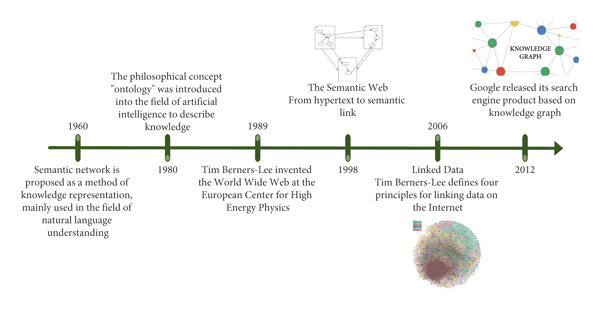
\includegraphics[height=1.00in,width=2.50in,viewport=0 0 160 75,clip]{Figures/Development-history-of-the-knowledge-graph.jpg}
\caption{\tiny\textrm{Schematic representation of the development history of the Knowledge Graph.}}%(与文献\cite{EPJB33-47_2003}图1对比)
\label{Fig:Knowledge-history}
\end{figure}
}

\frame
{
	\frametitle{知识图谱的要素}
知识图谱以图形结构的方式,通常使用节点(实体)和连线/边(关系)的形式表示知识\\
这种结构使得知识点之间的关联关系更加清晰和可视化

主要的关键词为:
\begin{itemize}
	\item 实体\textrm{(Entities)}:~知识图谱中的实体是指具体的事物、概念、人物、地点等,每个实体都有一个唯一的标识符\\
		例如,在化学知识图谱中,分子、合成体、密度等都是实体。
	\item 关系\textrm{(Relationships)}:~实体之间的关系表示不同实体之间的连接或互动。这些关系可以是有向的或无向的,用于描述实体之间的各种联系\\
		如” 具有”、” 属于”、”值为” 等。
	\item 属性\textrm{(Attributes)}:~实体可以有一些描述性的属性,这些属性是与实体相关的额外信息\\
		例如,分子(实体)的属性,包括分子量、化合价、密度等。
\end{itemize}
}

\frame
{
	\frametitle{资源的描述}
\begin{figure}[h!]
\centering
\vskip -8pt
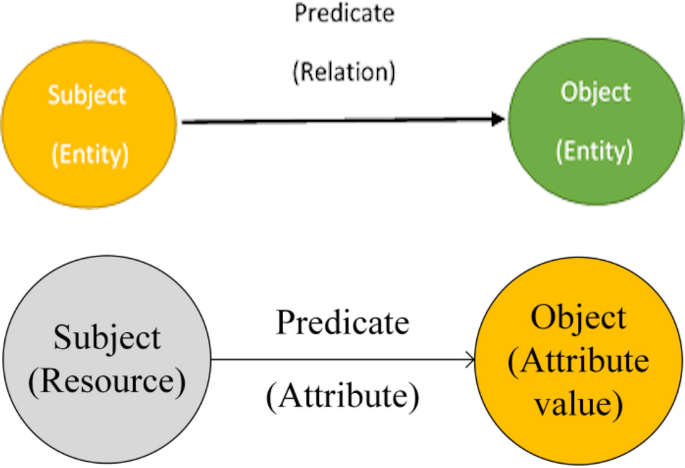
\includegraphics[height=2.35in,width=3.50in,viewport=0 0 690 470,clip]{Figures/KG-Entity-relation_0.png}
\caption{\tiny\textrm{Schematic representation of the relationship between entites.}}%(与文献\cite{EPJB33-47_2003}图1对比)
\label{Fig:KG-Entity-relations}
\end{figure}
}

\frame
{
	\frametitle{领域知识的描述:~\textrm{Ontology}}
	\textrm{Ontology}:~用于描述学科领域知识的通用概念模型,模型包含了学科内基本术语-术语间关系,是领域内概念的集合,\textcolor{blue}{属于群体概念}
	\begin{itemize}
		\item \textrm{Ontology}:~是哲学概念,哲学中关系的是客观存在的抽象本质
		\item 在语义学层次上,\textrm{Onlogy}是\textcolor{red}{共享概念模型的格式化规范说明}
	\begin{itemize}
		\item 共享\textrm{(Share)}:~知识必须是共同认可的
		\item 概念化\textrm{(Conceptualization)}:~对事物的描述构成一组概念
		\item 明确性\textrm{(Explicit)}:~每个术语、属性都有明确定义
		\item 格式化\textrm{(Format)}:~可以被计算机处理
	\end{itemize}
\item \textrm{Ontology}的描述语言主要有\textrm{RDF}、\textrm{RDFS}和\textrm{OWL}
	\begin{itemize}
		\item \textrm{RDF}:~用于描述\textrm{Web}上的资源\\
			用\textrm{Web}标识符来标记资源(主语),用属性(谓语)和属性值(宾语)来描述资源
		\item \textrm{RDFS}:~在\textrm{RDF}基础上扩展而成,更形象地表达知识
		\item \textrm{OWL}:~保持\textrm{RDF}、\textrm{RDFS}的兼容性,用于\textrm{ontology}的语义描述
	\end{itemize}
	\end{itemize}
}

\frame
{
	\frametitle{\textrm{RDF}举例:~分子与合成体的描述}
\begin{figure}[h!]
\centering
\vskip -8pt
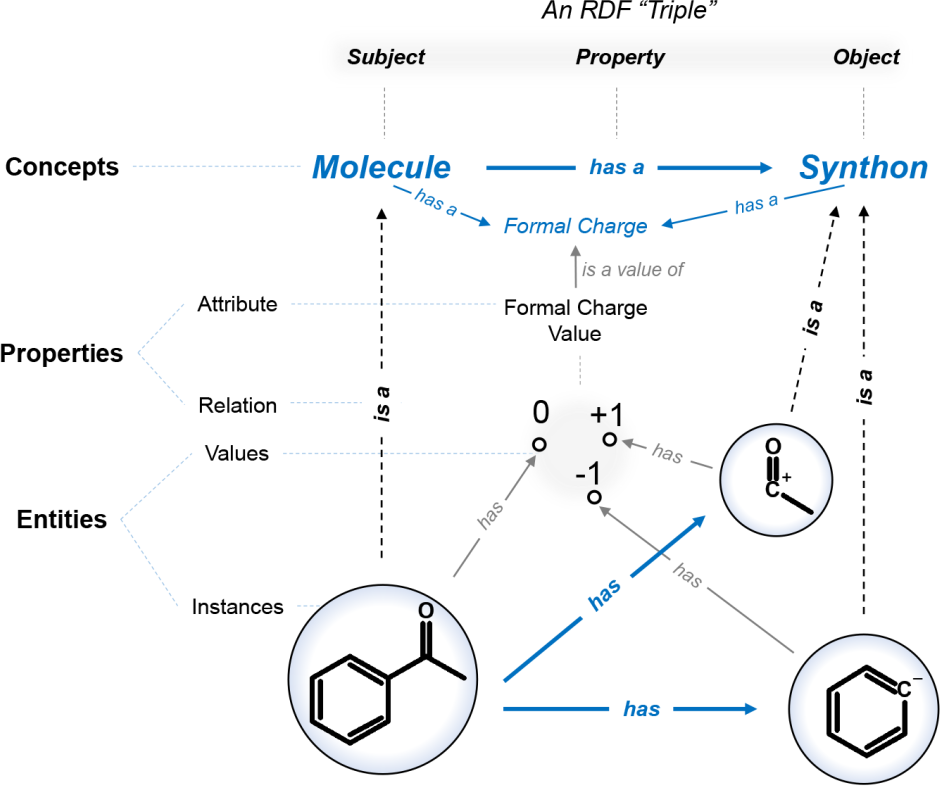
\includegraphics[height=2.60in,width=3.45in,viewport=0 0 950 790,clip]{Figures/Mapping-the-relationship-between-molecule-and-synthon.png}
\caption{\tiny\textrm{Mapping the relationship molecule (chemical) and synthon (abstract) concepts and illustrating them with instrances. cite from\cite{ACR56-128_2023}}}%(与文献\cite{EPJB33-47_2003}图1对比)
\label{Fig:Mapping-relationship-molecule-synthon}
\end{figure}
}

\begin{frame}
	\frametitle{数据:~一切知识的基础}
\begin{figure}[h!]
\centering
\vskip -8pt
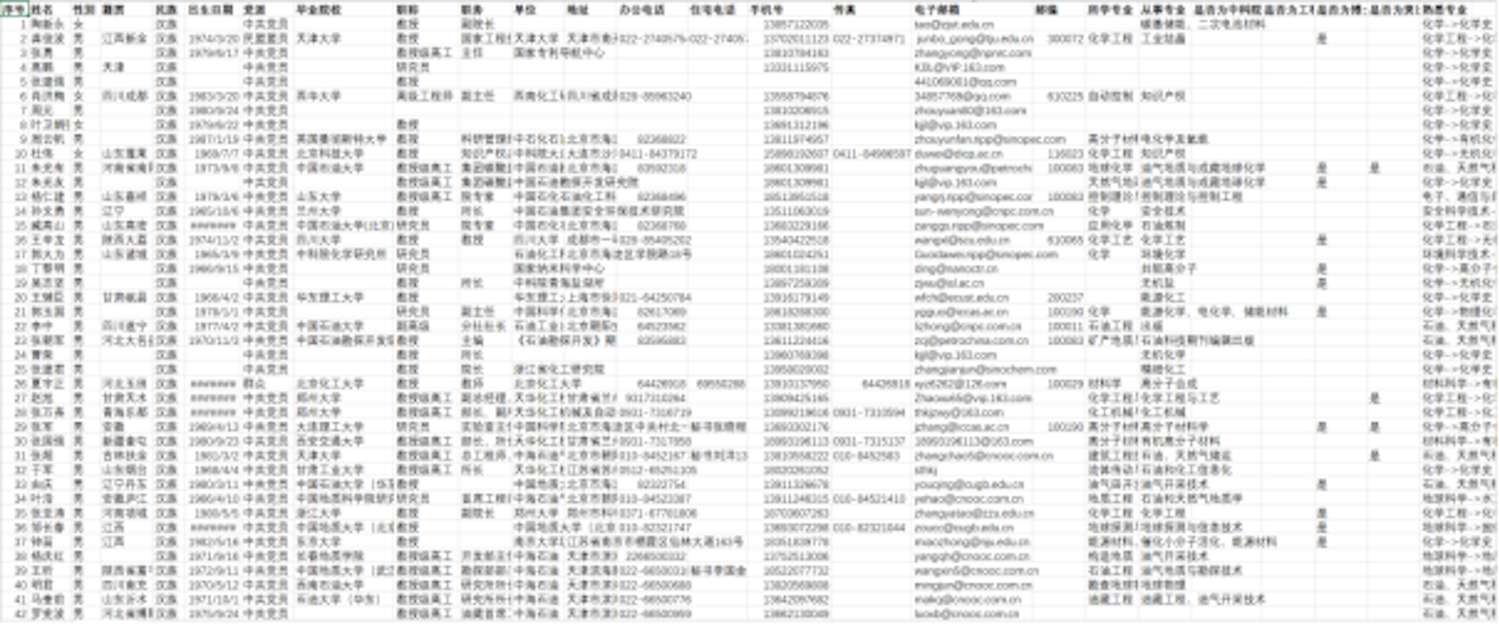
\includegraphics[height=2.10in,width=4.00in,viewport=0 0 360 160,clip]{Figures/KG_Chem-Info.png}
\caption{\tiny 有组织的数据是一切\textrm{AI}知识的基础}%(与文献\cite{EPJB33-47_2003}图1对比)
\label{Fig:KG_Chem-Enflurane}
\end{figure}
\end{frame}

\begin{frame}
	\frametitle{数据的提取}
\begin{figure}[h!]
\centering
%\vskip -8pt
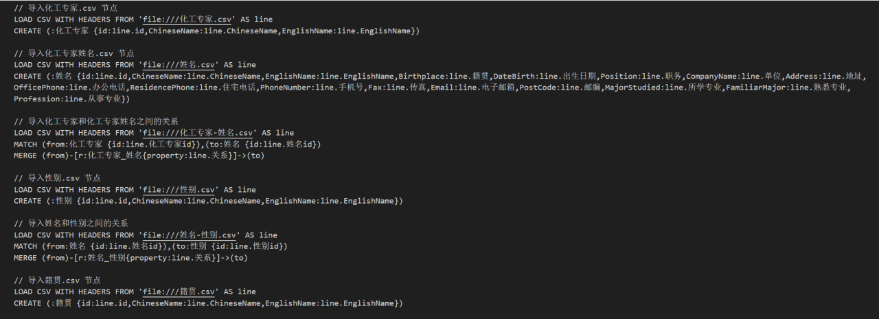
\includegraphics[height=2.10in,width=4.00in,viewport=0 0 240 130,clip]{Figures/KG_Chem-extract.png}
\caption{\tiny 数据的提取是一切\textrm{AI}知识分类的逻辑起点}%(与文献\cite{EPJB33-47_2003}图1对比)
\label{Fig:KG_Chem-Extract}
\end{figure}
\end{frame}

\subsection{化学-化工知识图谱}
\begin{frame}
	\frametitle{化学-化工知识图谱:~示例}
\begin{figure}[h!]
\centering
%\vskip -8pt
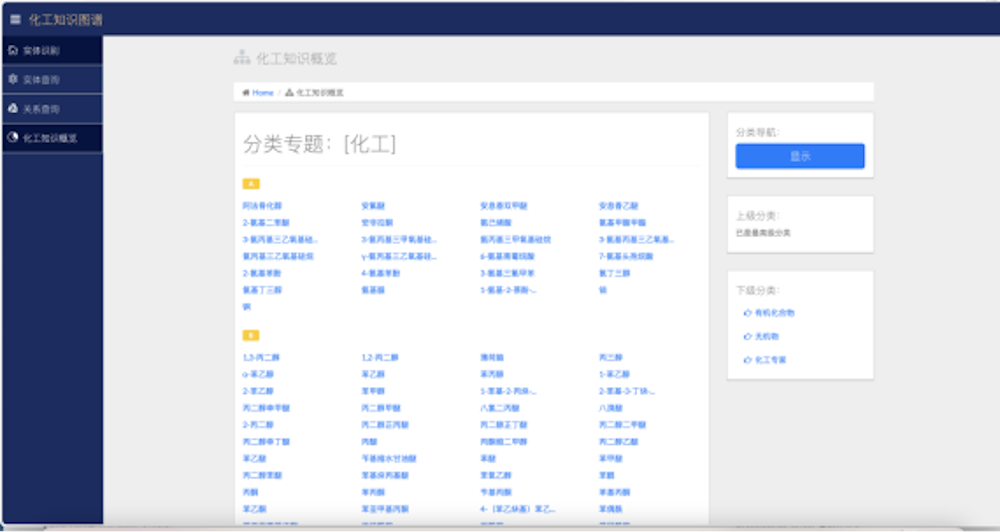
\includegraphics[height=2.10in,width=4.00in,viewport=0 0 240 130,clip]{Figures/KG_Chem-html.png}
\caption{\tiny 化学-化工知识图谱网页}%(与文献\cite{EPJB33-47_2003}图1对比)
\label{Fig:KG_Chem-Enflurane}
\end{figure}
\end{frame}

\begin{frame}
	\frametitle{化学-化工知识图谱:~示例}
\begin{figure}[h!]
\centering
%\vskip -8pt
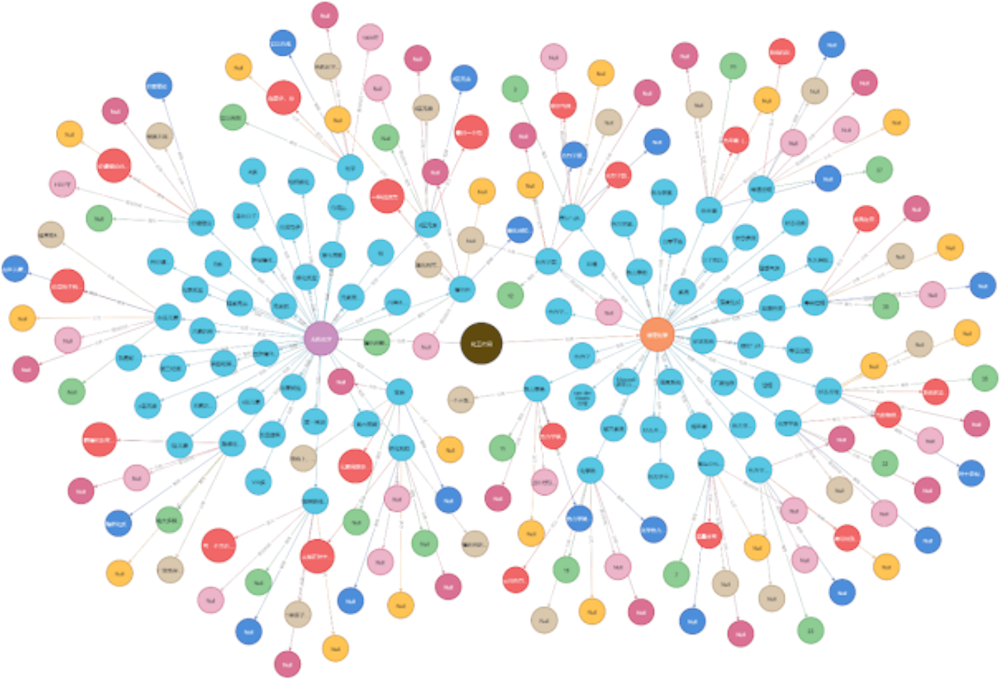
\includegraphics[height=2.60in,width=4.00in,viewport=0 0 240 180,clip]{Figures/KG_Chem-Inorganic.png}
\caption{\tiny 知识图谱的展示:~无机化合物}%(与文献\cite{EPJB33-47_2003}图1对比)
\label{Fig:KG_Chem-Inorganic}
\end{figure}
\end{frame}

\begin{frame}
	\frametitle{化学-化工知识图谱:~示例}
\begin{figure}[h!]
\centering
%\vskip -8pt
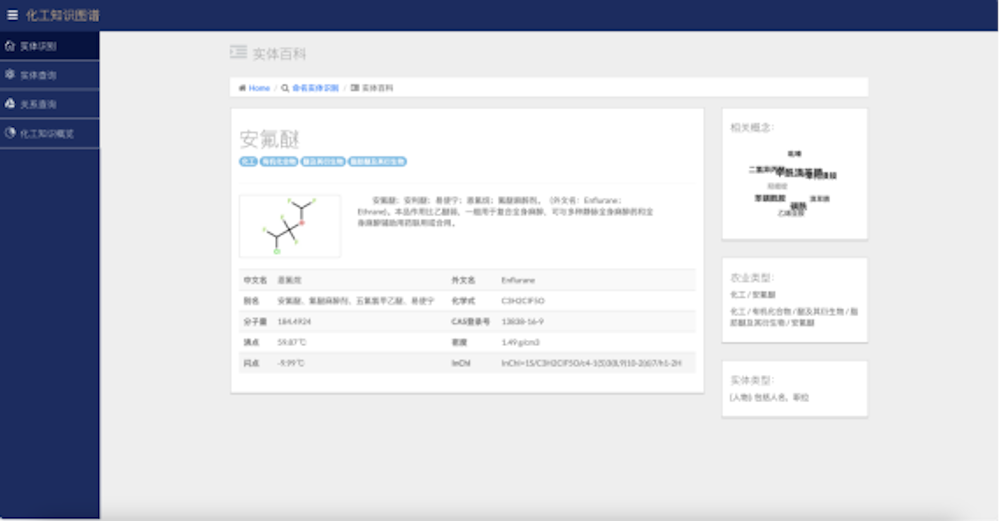
\includegraphics[height=2.20in,width=4.00in,viewport=0 0 240 130,clip]{Figures/KG_Chem-Enflurane.png}
\caption{\tiny 知识图谱的词条内容:~化合物\textrm{安氟醚}的有关知识}%(与文献\cite{EPJB33-47_2003}图1对比)
\label{Fig:KG_Chem-Enflurane}
\end{figure}
\end{frame}

%\frame
%{
%	\frametitle{化学-化工知识图谱的组成}
%\begin{figure}[h!]
%\centering
%\vskip -8pt
%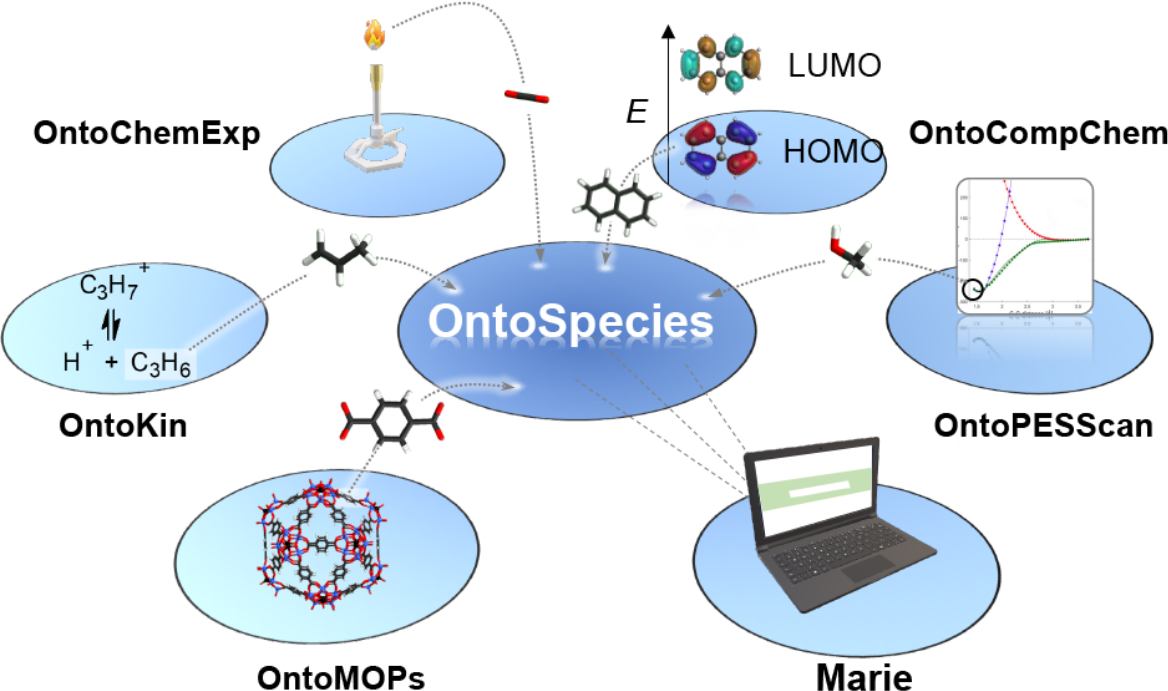
\includegraphics[height=2.45in,width=4.05in,viewport=0 0 1170 700,clip]{Figures/Connection-of-OntoSpecies-to-segments-of-KG.png}
%\caption{\tiny\textrm{Connection of OntoSpecies to other segments of TWA KG. cite from\cite{ACR56-128_2023}}}%(与文献\cite{EPJB33-47_2003}图1对比)
%\label{Fig:OntoSpecies-to-segments-TWA}
%\end{figure}
%}
%
%\frame
%{
%	\frametitle{化学-化工知识图谱}
%	化学-化工知识图谱:~以化学物种(元素、化合物)为核心的\textcolor{cyan}{多个知识的\textrm{Ontology}组成}
%	\begin{itemize}
%		\item \textrm{OntoSpecites}:~主要纪录化学物种的知识,包括分子式、电荷、分子量和自旋多重度等
%		\item \textrm{OntoKin}:~表示反应机理的知识,纪录反应物、产物和反应过程的信息
%		\item \textrm{OntoCompChem}:~表示计算化学的信息的知识,计算信息的描述包括
%			\begin{itemize}
%				\item 计算对象:~单点计算、结构优化和频率计算
%				\item 计算使用的软件,{\fontsize{7.2pt}{5.2pt}\selectfont{如\textrm{Gaussian~16}}}
%				\item 计算中使用的方法,包括泛函和基组{\fontsize{7.2pt}{5.2pt}\selectfont{~如\textrm{B3LYP,~6-31G(d)}}}
%				\item 电荷与自旋极化
%			\end{itemize}
%		\item \textrm{OntoCompExp}:~表示化学实验信息的知识,包括各类化学实验条件
%	\end{itemize}
%}
%
%\frame
%{
%	\frametitle{\textrm{OntoSpecies}:~化学物种的描述}
%\begin{figure}[h!]
%\centering
%\vskip -8pt
%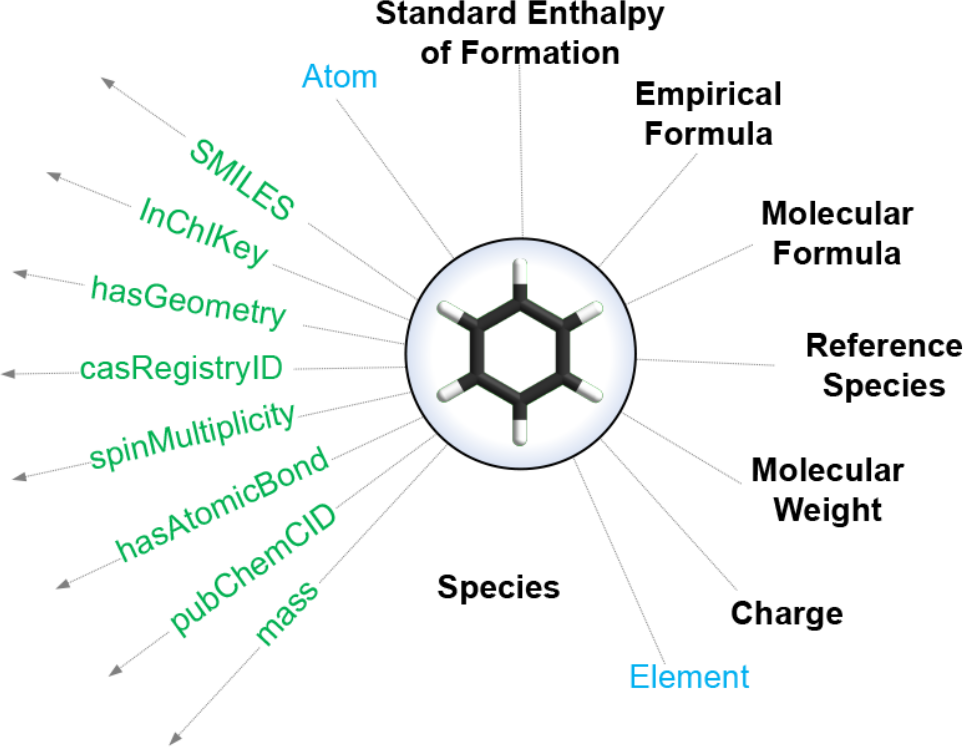
\includegraphics[height=2.40in,width=3.25in,viewport=0 0 990 750,clip]{Figures/Key_OntoSpecies-and-external_concepts.png}
%\caption{\tiny\textrm{Key OntoSpecies (black) and external (blue) concepts, along with a number of properties (green) used to describe chemical species in TWA KG. cite from\cite{ACR56-128_2023}}}%(与文献\cite{EPJB33-47_2003}图1对比)
%\label{Fig:Key-OntoSpecies-and-external-concepts}
%\end{figure}
%}
%
%\frame
%{
%	\frametitle{\textrm{Agent}:~化学-化工知识图谱的组织工具}
%	\textrm{Agent}:~能够感知环境、进行决策和执行动作的智能处理软件
%	\begin{itemize}
%		\item \textrm{Agent}工作方式类似于人类代理:~能接收输入数据(如传感器信息、文本、图像等),通过分析和处理数据,理解环境和任务要求,并做出相应的决策和行动
%		\item 应用场景广泛,如自动驾驶车辆、智能机器人、语音助手等
%		\item \textrm{Agent}核心功能:~感知、推理和决策
%			\begin{itemize}
%				\item 感知:~通过传感器等方式获取环境信息的能力,例如通过摄像头获取图像或通过麦克风获取声音
%				\item 推理:~基于获取的信息进行逻辑推理和分析的能力,以了解环境和任务需求
%				\item 决策:~根据推理结果做出相应的决策,并执行相应的动作
%			\end{itemize}
%		\item 通过与环境的交互和反馈,\textrm{Agent}可以逐步改进性能和表现,实现好的任务执行能力\\
%		\item \textrm{Agent}设计和训练,需要结合机器学习和人工智能技术,如强化学习、深度学习等
%	\end{itemize}
%}
%
%\frame
%{
%	\frametitle{知识图谱组织示例}
%\begin{figure}[h!]
%\centering
%\vskip -8pt
%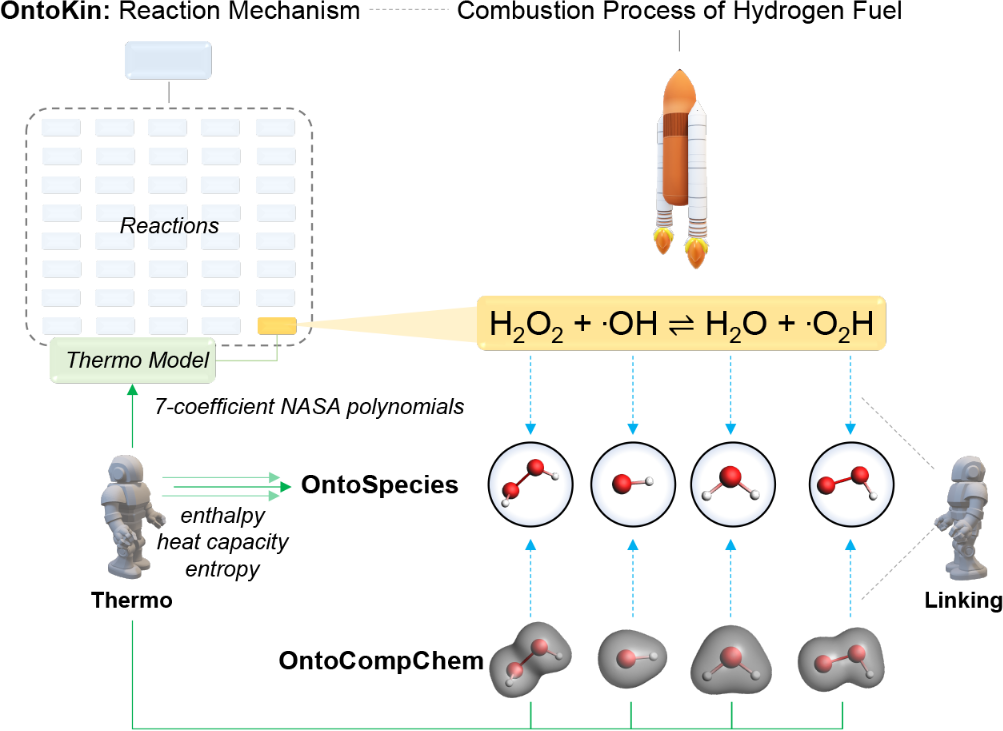
\includegraphics[height=2.70in,width=3.75in,viewport=0 0 1010 750,clip]{Figures/Automated-linking-between-OntoSepcies-Kin-CompChem.png}
%\caption{\tiny\textrm{Automated linking between OntoSpecies, OntoKin and OntoCompChem. cite from\cite{ACR56-128_2023}}}%(与文献\cite{EPJB33-47_2003}图1对比)
%\label{Fig:Automated-linking-between-OntoSpecies-Kin-CompChem}
%\end{figure}
%}
%
%\frame
%{
%	\frametitle{知识图谱组织示例}
%\begin{figure}[h!]
%\centering
%\vskip -8pt
%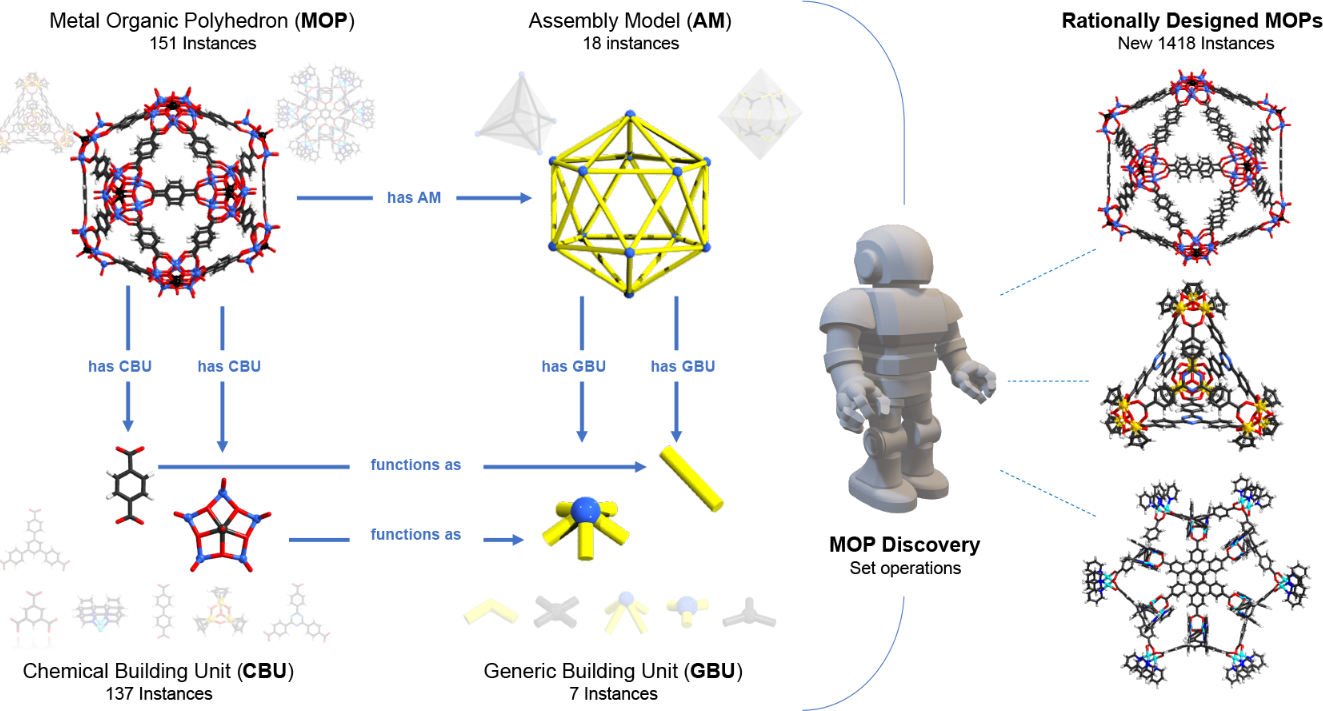
\includegraphics[height=2.20in,width=4.05in,viewport=0 0 1330 700,clip]{Figures/Key_concepts-in-OntoMOPs-and-designed-MOPs.png}
%\caption{\tiny\textrm{Key concepts in OntoMOPs (left) and examples of newly rationally designed MOPs (right). cite from\cite{ACR56-128_2023}}}%(与文献\cite{EPJB33-47_2003}图1对比)
%\label{Fig:OntoMOPs-MOPs}
%\end{figure}
%}

%\begin{frame}
%	\frametitle{应用:~类石墨烯材料的稳定性优化预测}
%\begin{figure}[h!]
%\centering
%%\hskip -35pt
%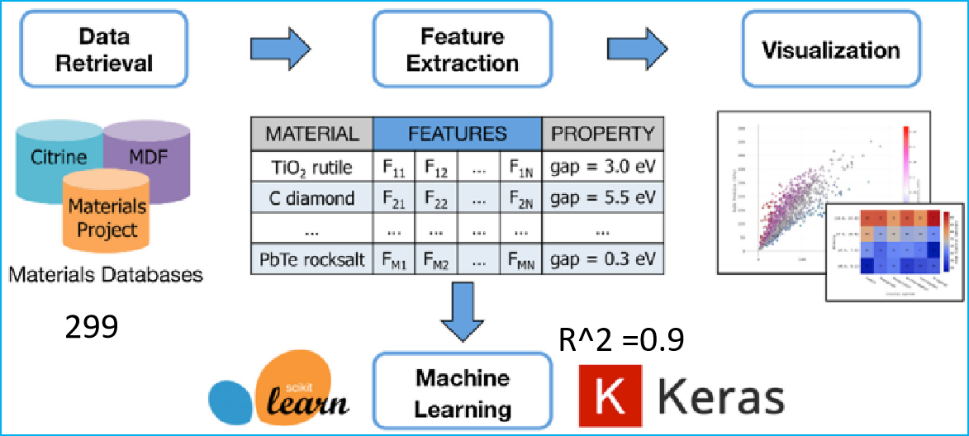
\includegraphics[height=1.55in]{Figures/MP_comp_BCC-5.png}
%%\caption{\fontsize{6.5pt}{4.5pt}\selectfont{面向多尺度材料智能计算平台}}%
%\label{MP_comp_BCC_5}
%\end{figure}
%{\fontsize{7.5pt}{5.5pt}\selectfont{
%	\begin{itemize}
%		\item 应用高通量建模软件构建潜在构型5600多种,利用\textrm{Materials~Projects}材料计算数据库提取竞争相数据
%		\item 通过热分解过程,组合化学反应式2000多组,筛选出热力学稳定的材料299种
%		\item 通过支持向量、高斯过程、随机深林、神经网络以及\textrm{adaboost}多种机器学习回归模型,利用13种常见特征参数对稳定性做了预测
%		\item 预测准确率达到94\%,节省计算成本高达70\%
%	\end{itemize}}}
%\end{frame}
%
%\begin{frame}
%	\frametitle{应用:~监督学习预测半导体材料带隙}
%\begin{figure}[h!]
%\centering
%\hspace*{-8pt}
%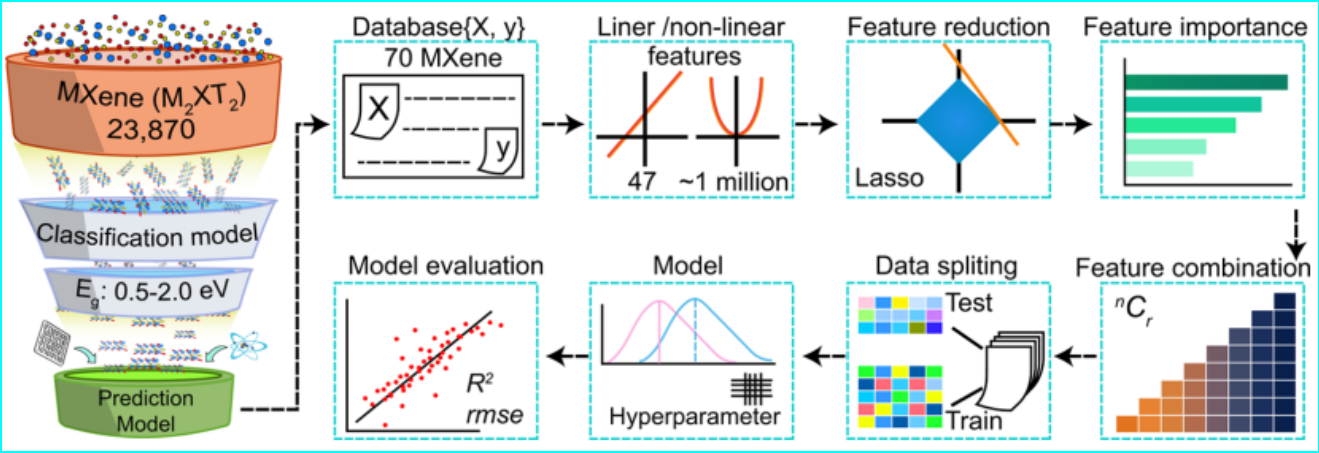
\includegraphics[height=1.45in]{Figures/MP_comp_BCC-6.png}
%%\caption{\fontsize{6.5pt}{4.5pt}\selectfont{面向多尺度材料智能计算平台}}%
%\label{MP_comp_BCC_6}
%\end{figure}
%{\fontsize{7.5pt}{5.5pt}\selectfont{
%	\begin{itemize}
%		\item 常规通行的材料模拟中带隙计算相当耗时
%		\item 利用%类石墨烯新能源
%	材料高通量智能计算与多目标机器学习集成研发平台,高通量自动化快速构建类石墨烯材料结构23870种,并构建数据库结合\textrm{KRR}、\textrm{SVR}、\textrm{GPR}、\textrm{Bagging}机器学习回归模型进行训练预测
%		\item \textrm{GPR}方法预测准确性达到了97\%,可以节省计算成本90\%多
%	\end{itemize}}}
%\end{frame}

%\begin{frame}[allowframebreaks]
%	\frametitle{主要合作与推广应用}
%		中科合成油(合作)
%	\begin{itemize}
%	 \setlength{\itemsep}{30pt}
%	\item 化学-化工知识图谱的建设
%\begin{figure}[h!]
%\centering
%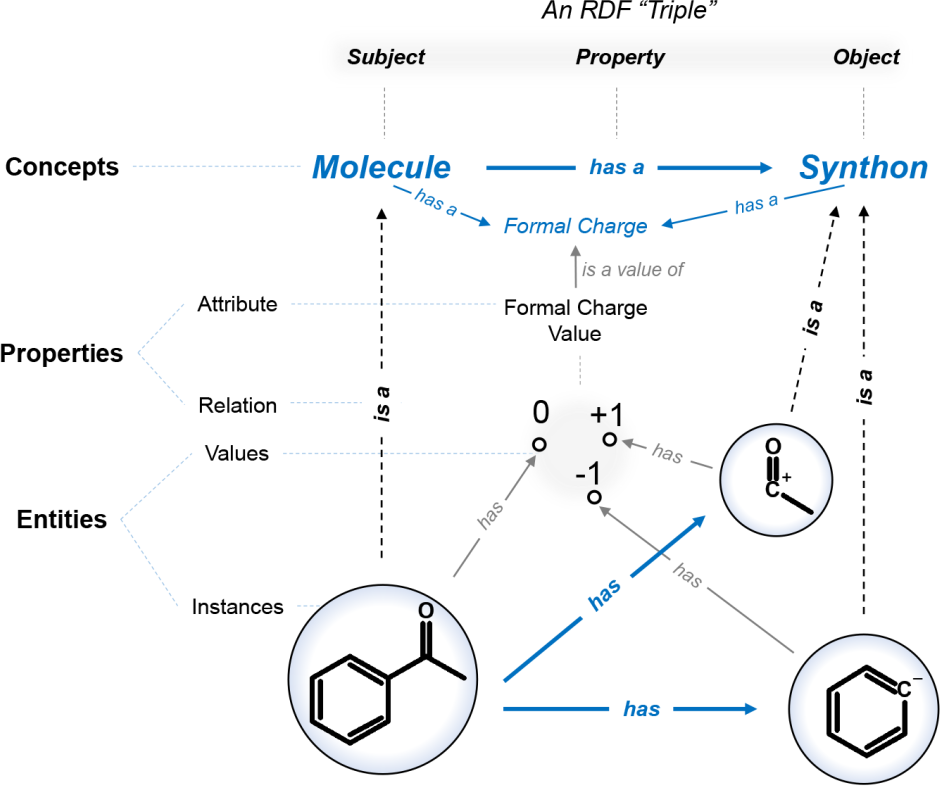
\includegraphics[height=1.50in,width=1.75in,viewport=0 0 950 790,clip]{Figures/Mapping-the-relationship-between-molecule-and-synthon.png}
%\hspace{5pt}
%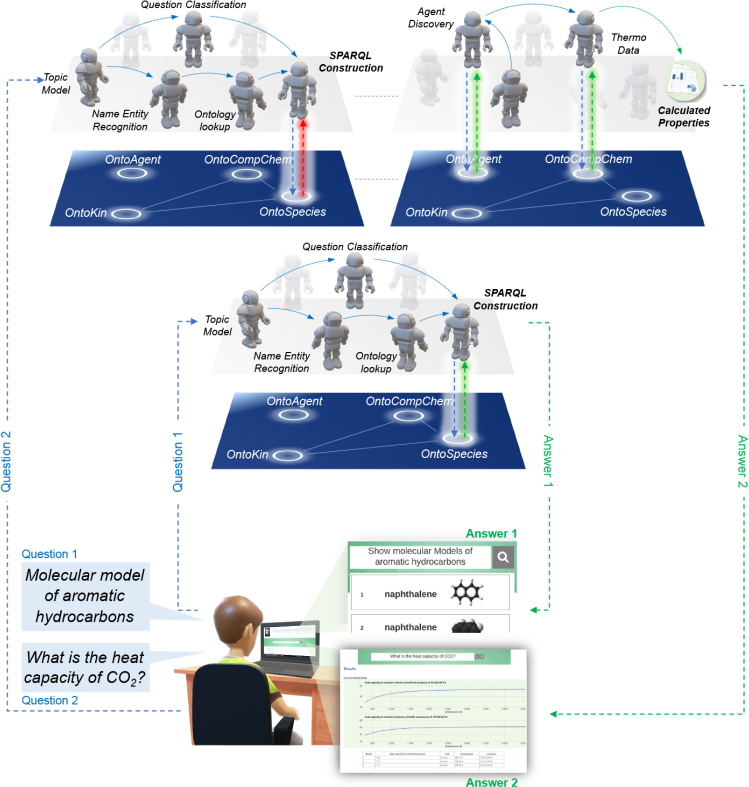
\includegraphics[height=1.50in,width=1.55in,viewport=0 0 750 790,clip]{Figures/TWA-KG-Marie.png}
%%\caption{\small\textrm{Mapping the relationship molecule (chemical) and synthon (abstract) concepts and illustrating them with instrances. cite from\cite{ACR56-128_2023}}}%(与文献\cite{EPJB33-47_2003}图1对比)
%\label{Fig:Mapping-relationship-molecule-synthon}
%\end{figure}
%	\begin{itemize}
%{\fontsize{7.5pt}{5.5pt}\selectfont{
%		\item 以化合物为核心,借助语义网\textrm{(Semantic Web)},组织、表示和存储化学-化工和领域特定类型的知识
%		\item 构建拥有学习和推理能力,具备初级的创造知识的能力}}
%	\end{itemize}
%	\item 问-答式煤化工智能模型建设
%\begin{figure}[h!]
%\centering
%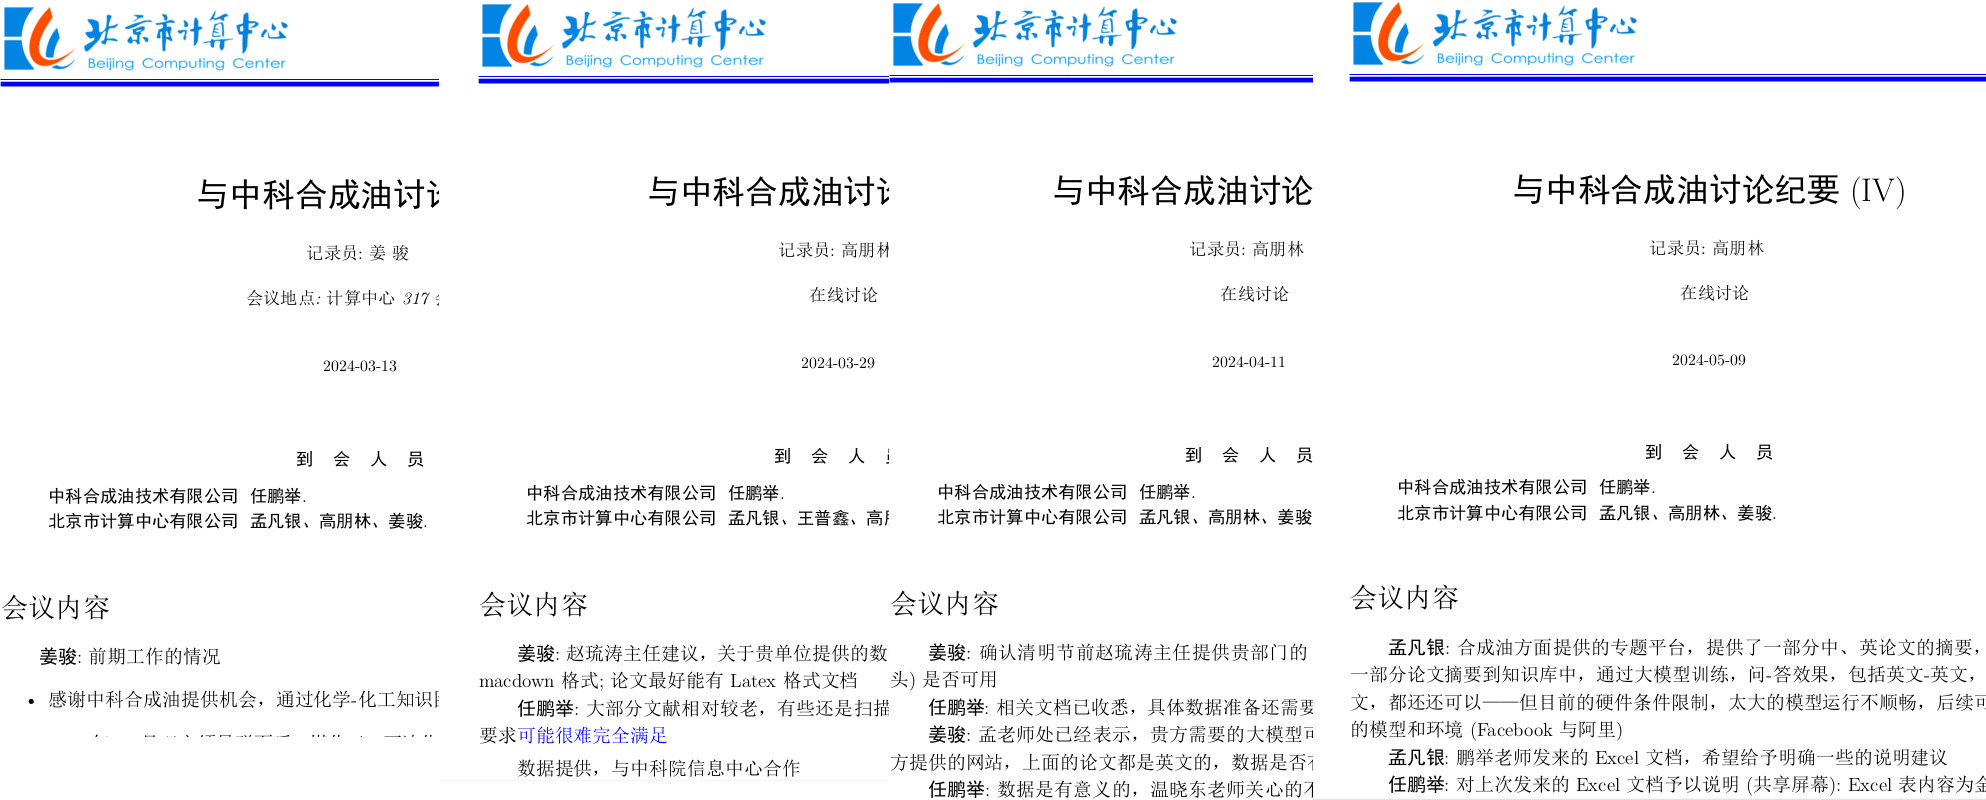
\includegraphics[height=1.40in,width=3.50in,viewport=0 0 1986 800,clip]{Figures/MeetingRecord_SCTC-BCC.png}
%\label{Fig:Meeting_Record}
%\end{figure}
%\begin{itemize}
%	\item 面向人工智能的全方位转型:\\
%		面向碳基础材料、发挥人工智能的作用
%	\item 大模型加持专业知识
%\end{itemize}
%	\end{itemize}
%\textcolor{purple}{目标:}~智能实验室-智能科学家
%\end{frame}
%
%\begin{frame}
%	\frametitle{数据驱动的材料研发:~应用前景}
%	\begin{enumerate}
%	 \setlength{\itemsep}{20pt}
%	 \item 航空发动机材料:~\textcolor{blue}{镍基单晶高温合金材料}\\
%	合金组分优化与强化功能提升
%
%\item 煤化工催化材料:~\textcolor{blue}{新型铁触媒材料}\\
%	反应活化性能提升与化学平衡的移动
%
%		\item 稀土功能材料:~\textcolor{blue}{钕铁硼永磁材料},\textcolor{blue}{稀土发光材料}\\
%	3\textit{d}-4\textit{f} 电子相互作用机制的认知
%
%	\end{enumerate}
%
%	\textcolor{magenta}{材料组分趋于复杂、材料机理认知趋于微观、材料与数据趋于膨胀}
%%\begin{figure}[h!]
%%\vspace*{-0.20in}
%%\centering
%%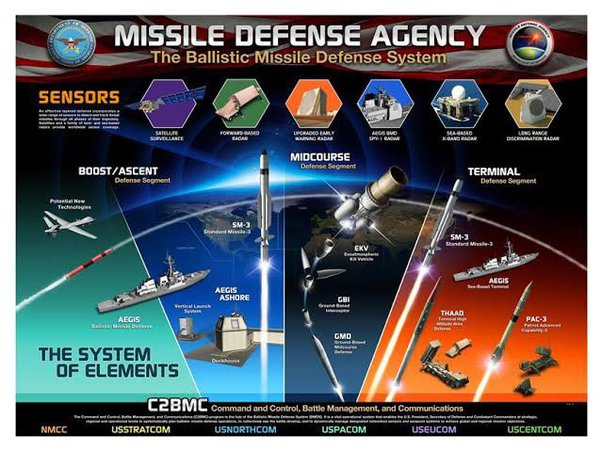
\includegraphics[height=2.90in,width=3.70in]{Figures/Main-qimg.jpeg}
%%\label{BMDS}
%%\end{figure}
%\end{frame}
\section{\rm{AI}大模型}
\subsection{通用语义大模型的搭建}
\begin{frame}
	\frametitle{知识问答大模型的搭建}
\begin{figure}[h!]
\centering
\vskip -8pt
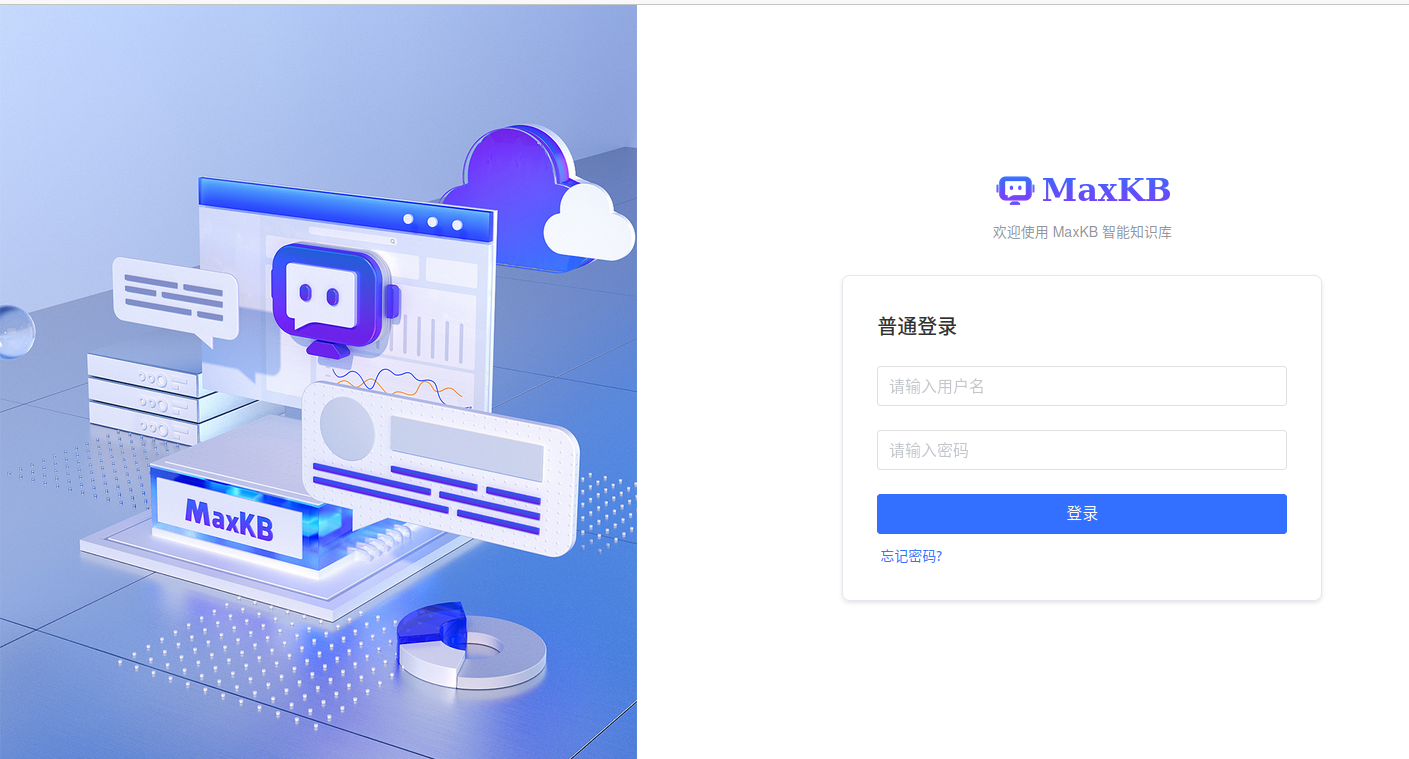
\includegraphics[height=1.90in,width=3.75in,viewport=0 0 1409 750,clip]{Figures/MaxKB_login.png}
\caption{\tiny\textrm{The login of MaxKB}}%(与文献\cite{EPJB33-47_2003}图1对比)
\label{Fig:MaxKB_login}
\end{figure}
{\fontsize{7.5pt}{6.0pt}\selectfont{化学-化工知识助手基于通用的\textrm{MaxKB}大模型知识问答系统搭建 (当前通用模型大小约\textrm{13TB}),主要通过对中科合成油提供的数据(主要是文献,约\textrm{500}篇)的学习,训练面向煤化工研究的专业知识问-答模型}}
\end{frame}

\begin{frame}
	\frametitle{知识问答大模型的搭建}
\begin{figure}[h!]
\centering
\vskip -8pt
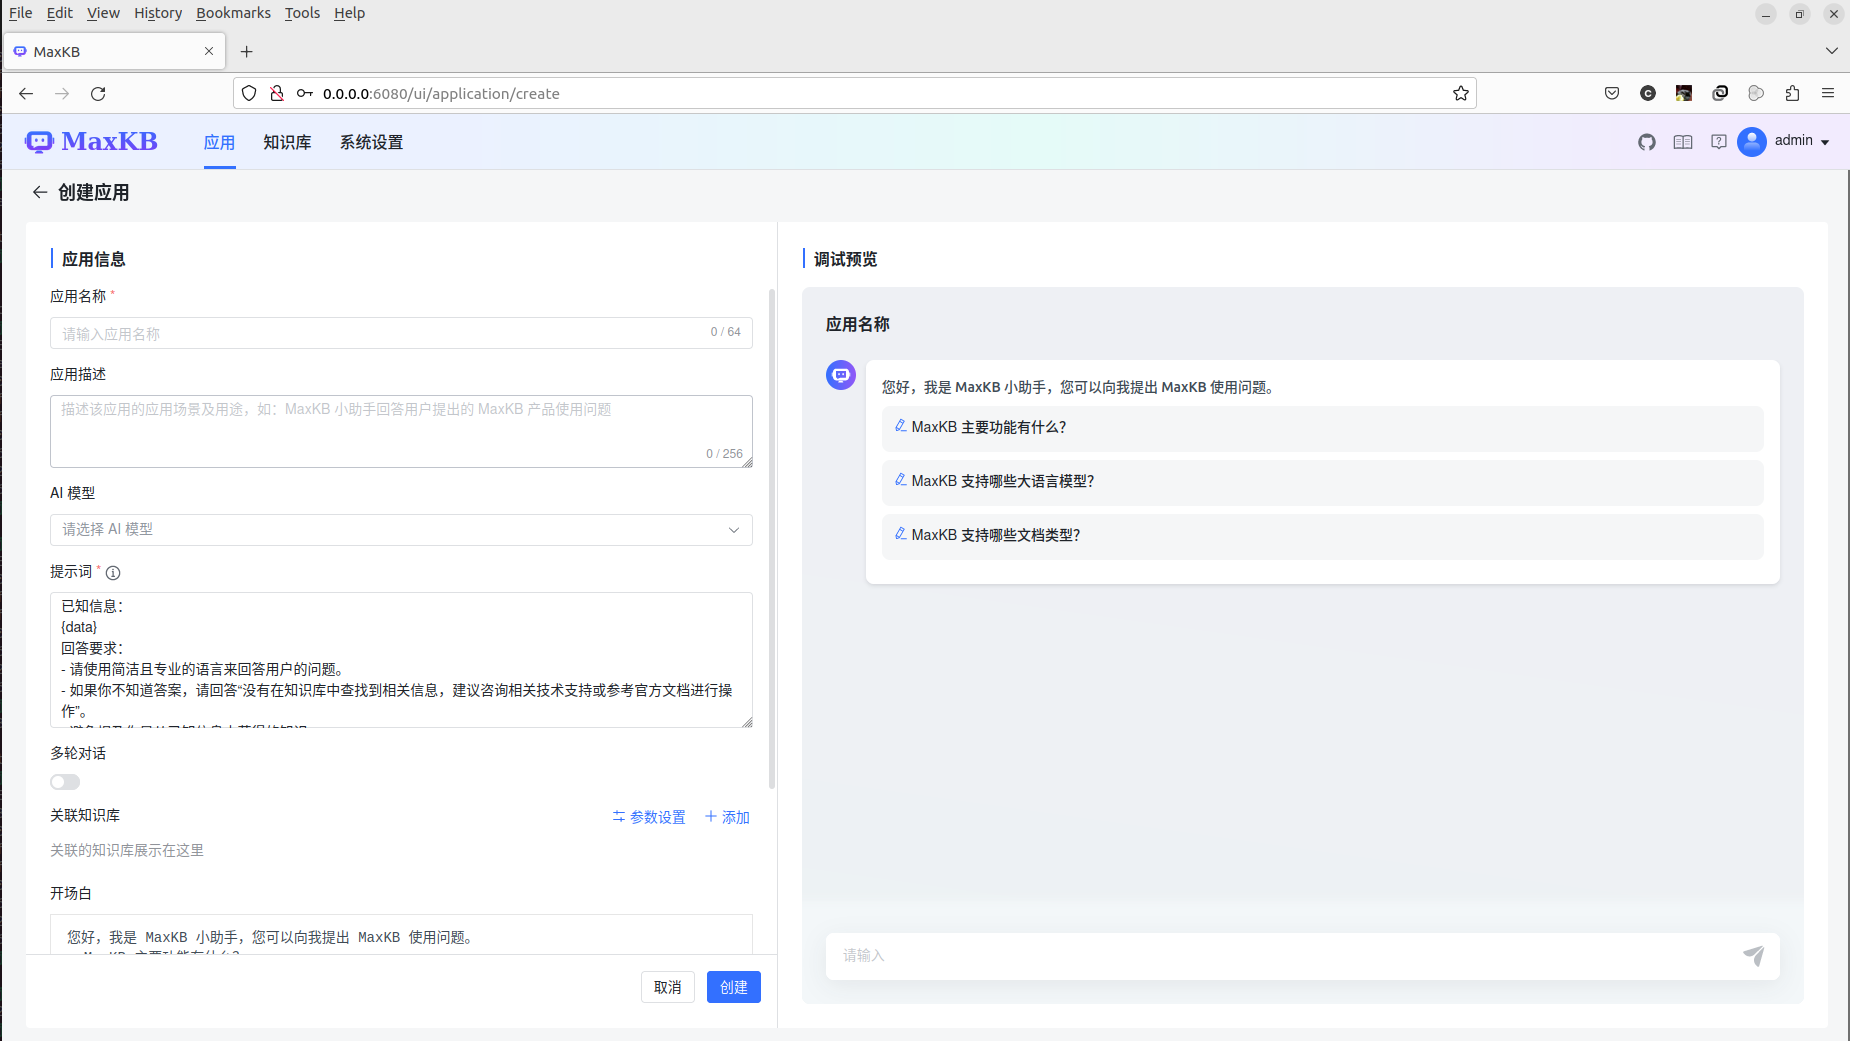
\includegraphics[height=2.2in,width=3.90in,viewport=3 0 1848 1041,clip]{Figures/MaxKB_Creat-APP.png}
\caption{\tiny\textrm{The Configuration of MaxKB}}%(与文献\cite{EPJB33-47_2003}图1对比)
\label{Fig:MaxKB_Creat-APP}
\end{figure}
\end{frame}

\begin{frame}
	\frametitle{知识问答大模型的搭建}
\begin{figure}[h!]
\centering
\vskip -8pt
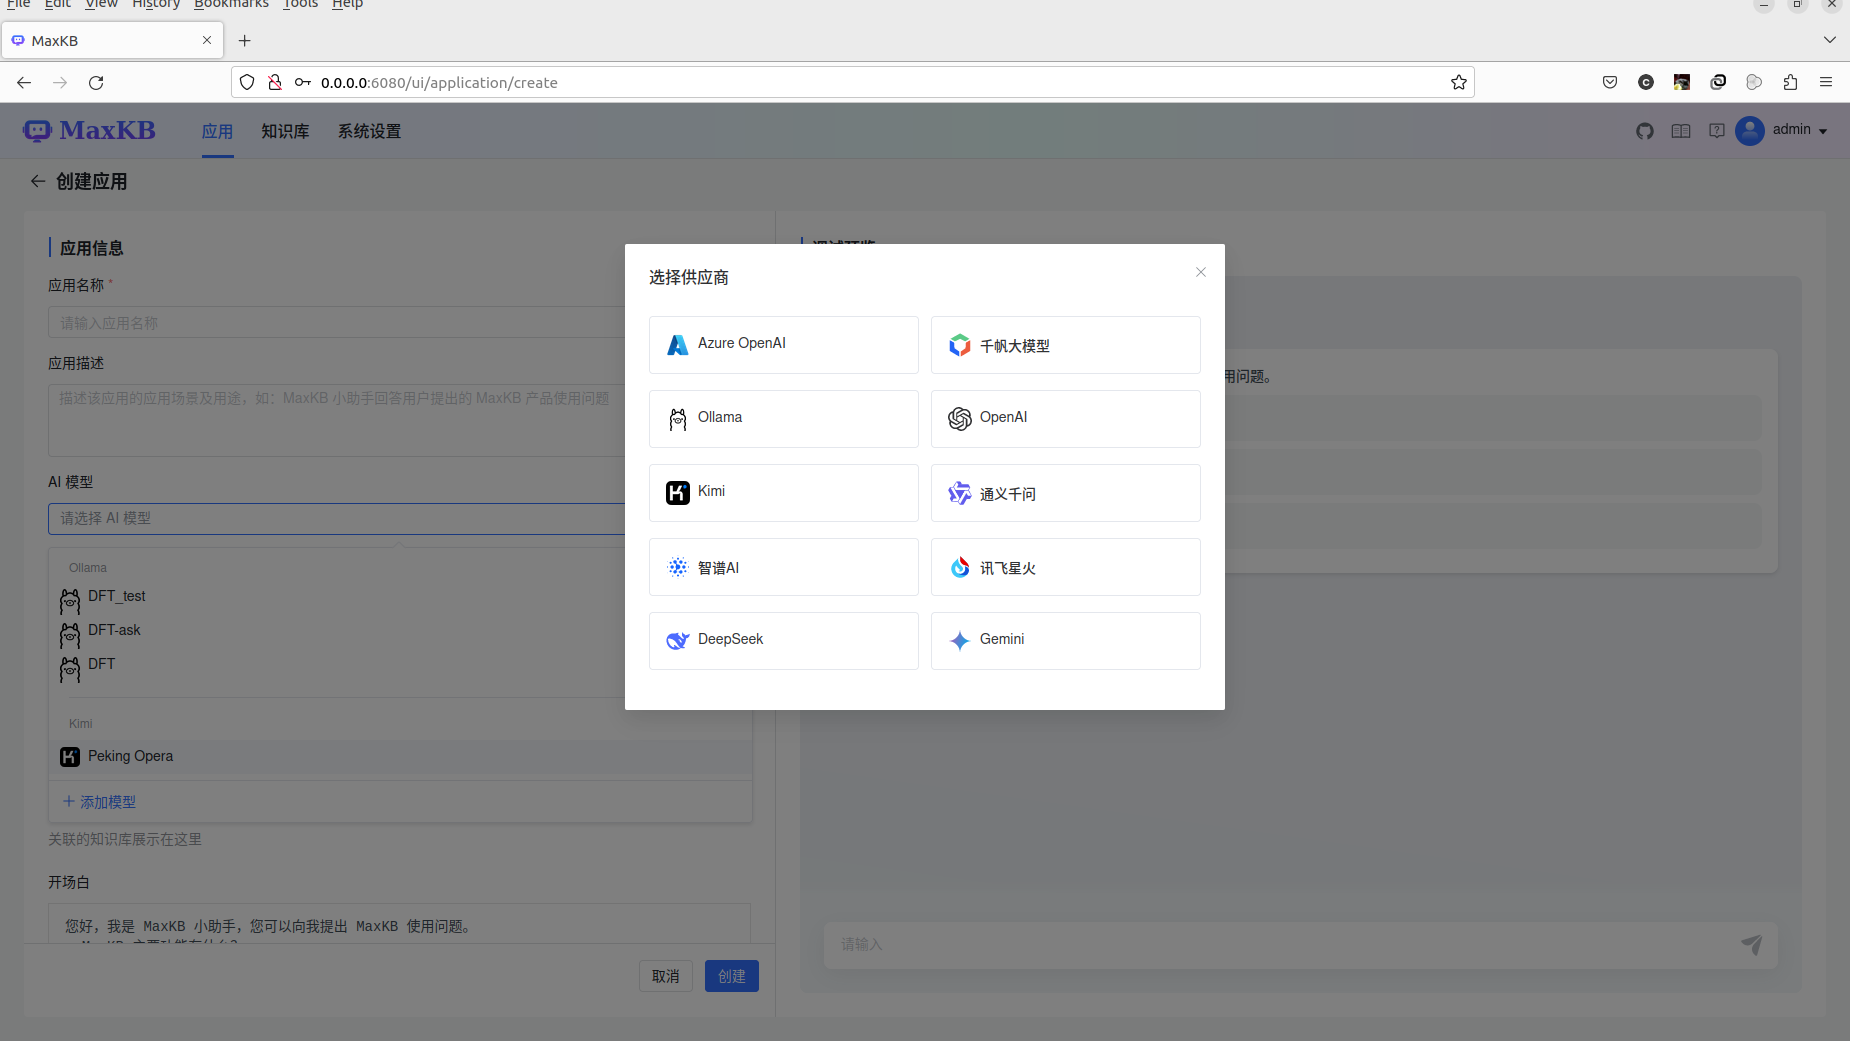
\includegraphics[height=2.20in,width=3.90in,viewport=0 0 1850 1041,clip]{Figures/MaxKB_Chose-Model.png}
\caption{\tiny\textrm{The Configuration of MaxKB}}%(与文献\cite{EPJB33-47_2003}图1对比)
\label{Fig:MaxKB_Chose-Model}
\end{figure}
\end{frame}

\begin{frame}
	\frametitle{知识问答大模型的搭建}
\begin{figure}[h!]
\centering
\vskip -8pt
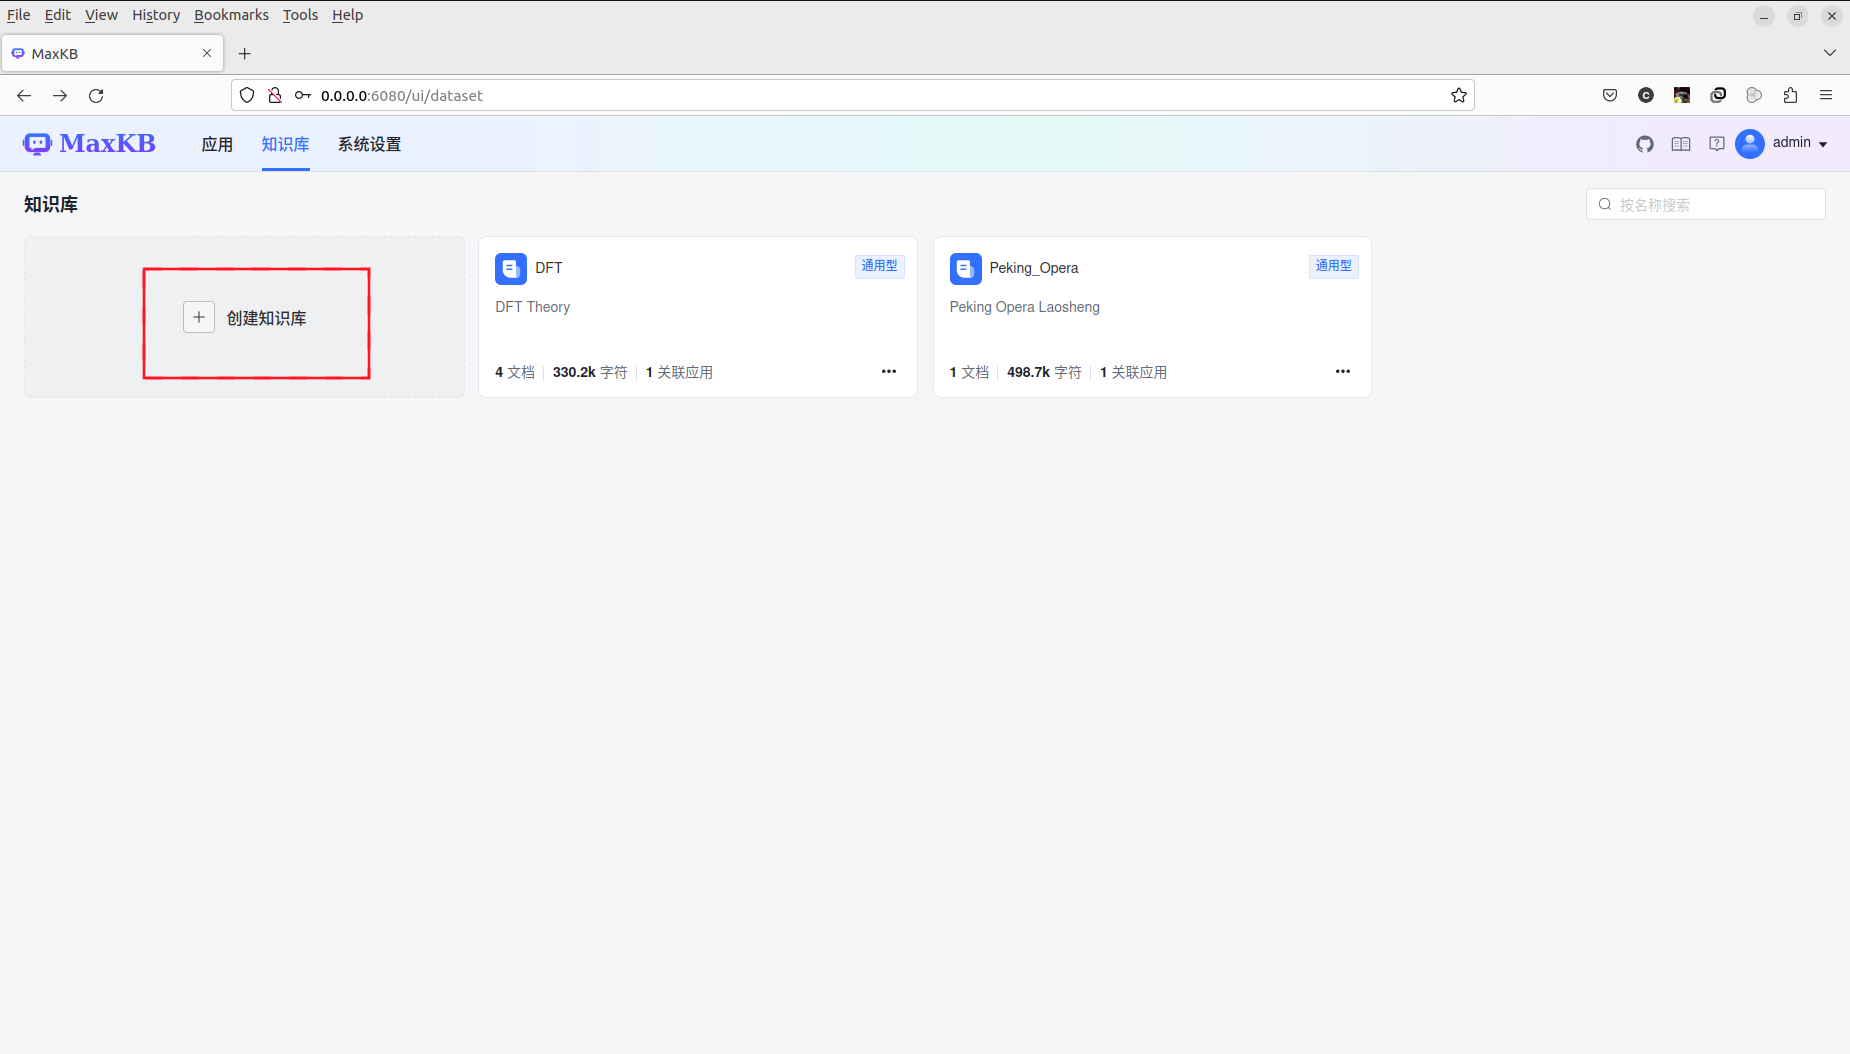
\includegraphics[height=0.80in,width=3.90in,viewport=0 650 1850 1054,clip]{Figures/MaxKB_NewDatabase.png}
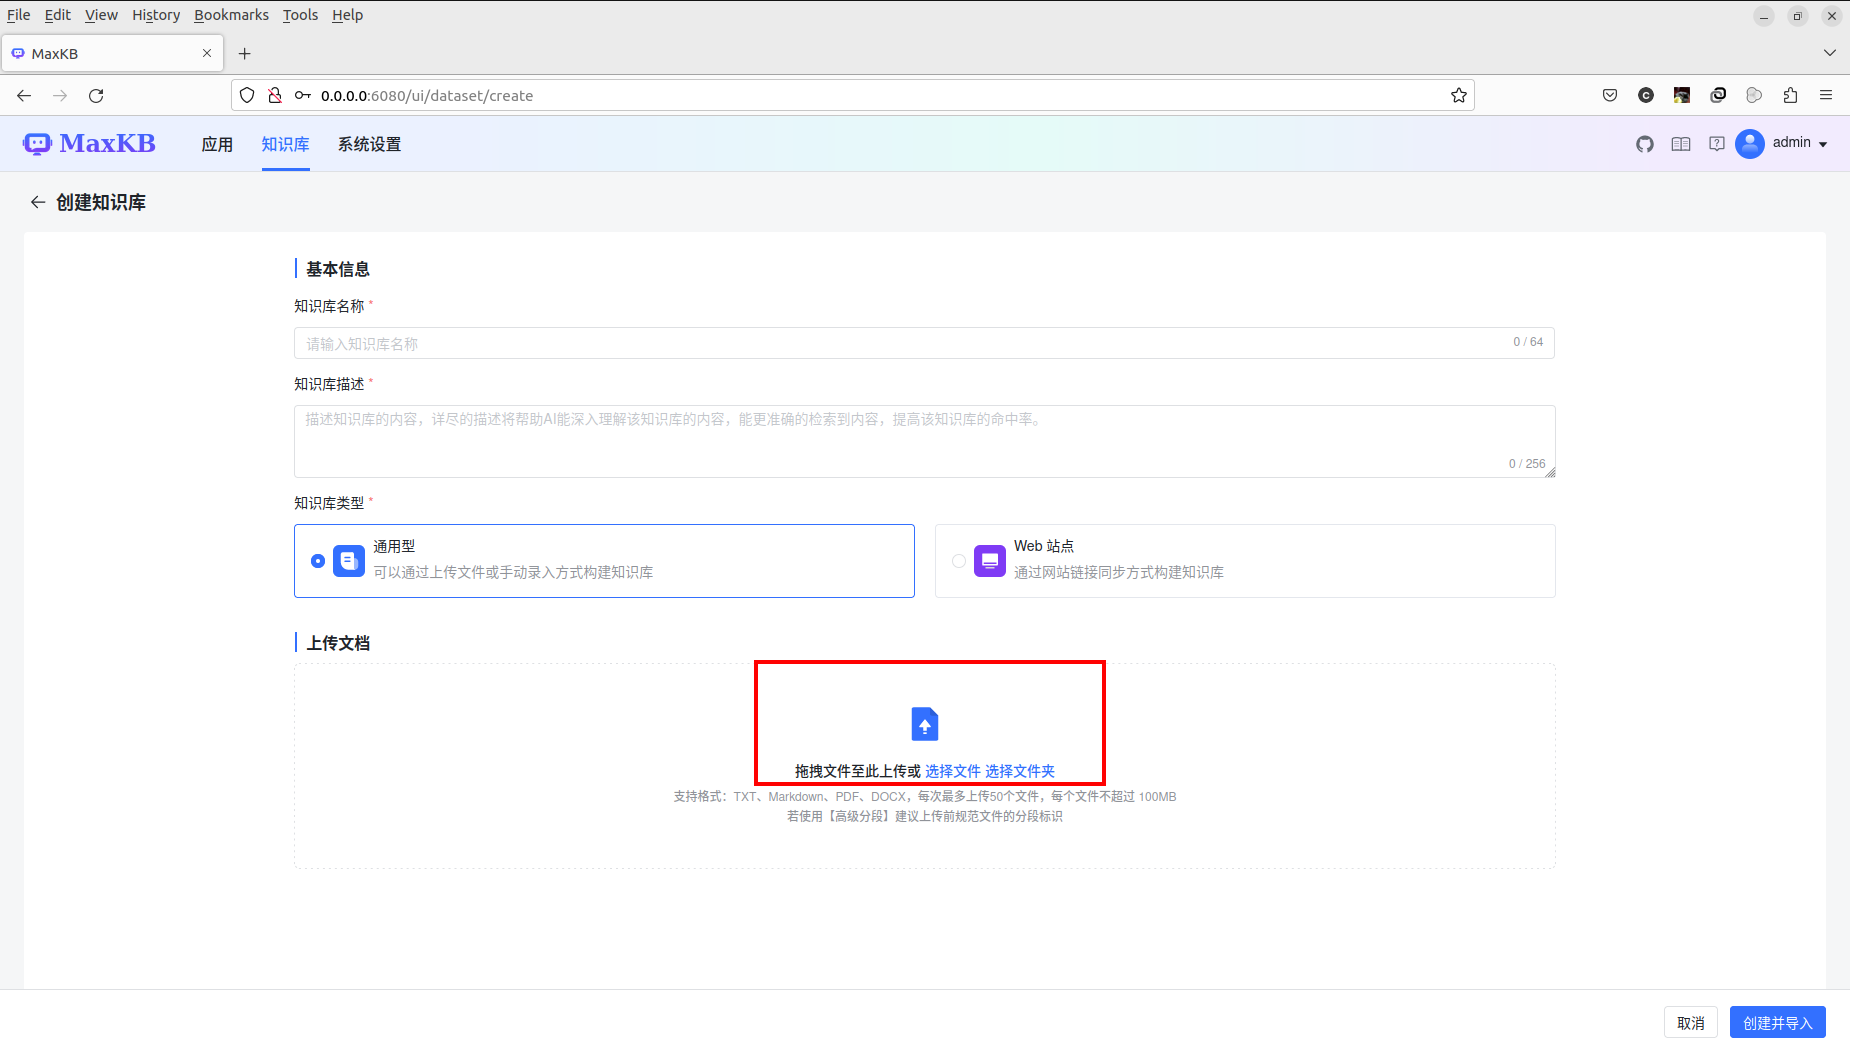
\includegraphics[height=1.80in,width=3.90in,viewport=0 0 1850 880,clip]{Figures/MaxKB_Database.png}
\caption{\tiny\textrm{Uploading a New File to the Database}}%(与文献\cite{EPJB33-47_2003}图1对比)
\label{Fig:MaxKB_Database}
\end{figure}
\end{frame}

\subsection{化学-化工知识问答}
\begin{frame}
	\frametitle{化学-化工知识的大模型数据}	
\begin{figure}[h!]
\centering
%\vskip -8pt
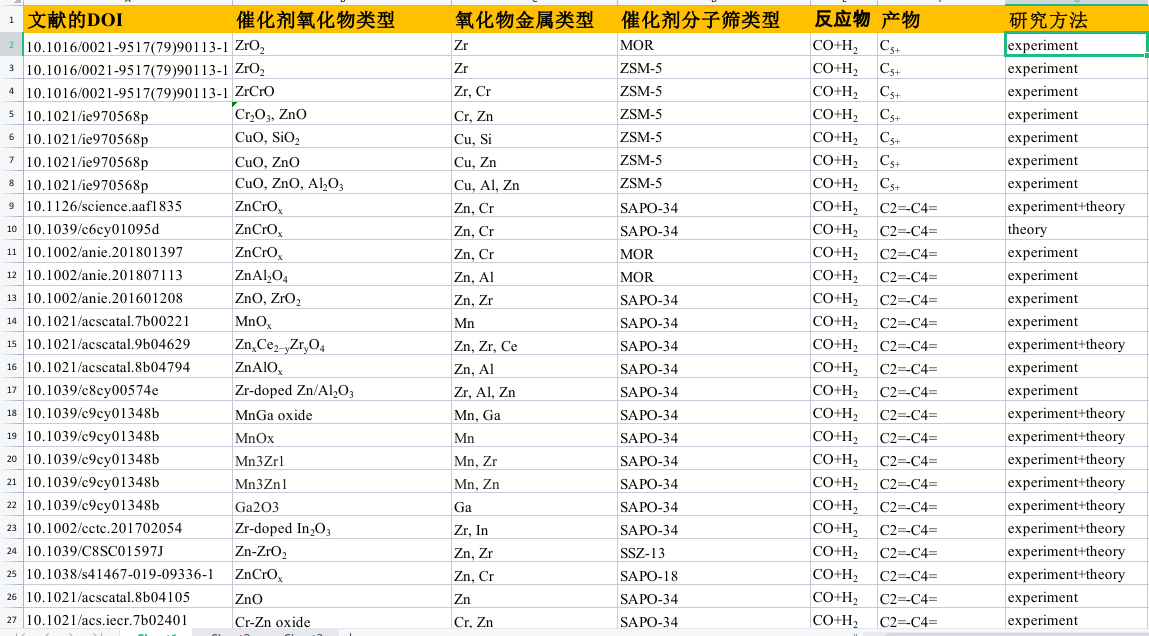
\includegraphics[height=2.10in,width=4.00in,viewport=0 0 1149 636,clip]{Figures/MaxKB_Info-1.png}
\caption{\tiny\textrm{Data uploaded for MaxKB}}%(与文献\cite{EPJB33-47_2003}图1对比)
\label{Fig:MaxKB_Data-1}
\end{figure}
\end{frame}

\begin{frame}
	\frametitle{化学-化工知识的大模型数据}	
\begin{figure}[h!]
\centering
%\vskip -8pt
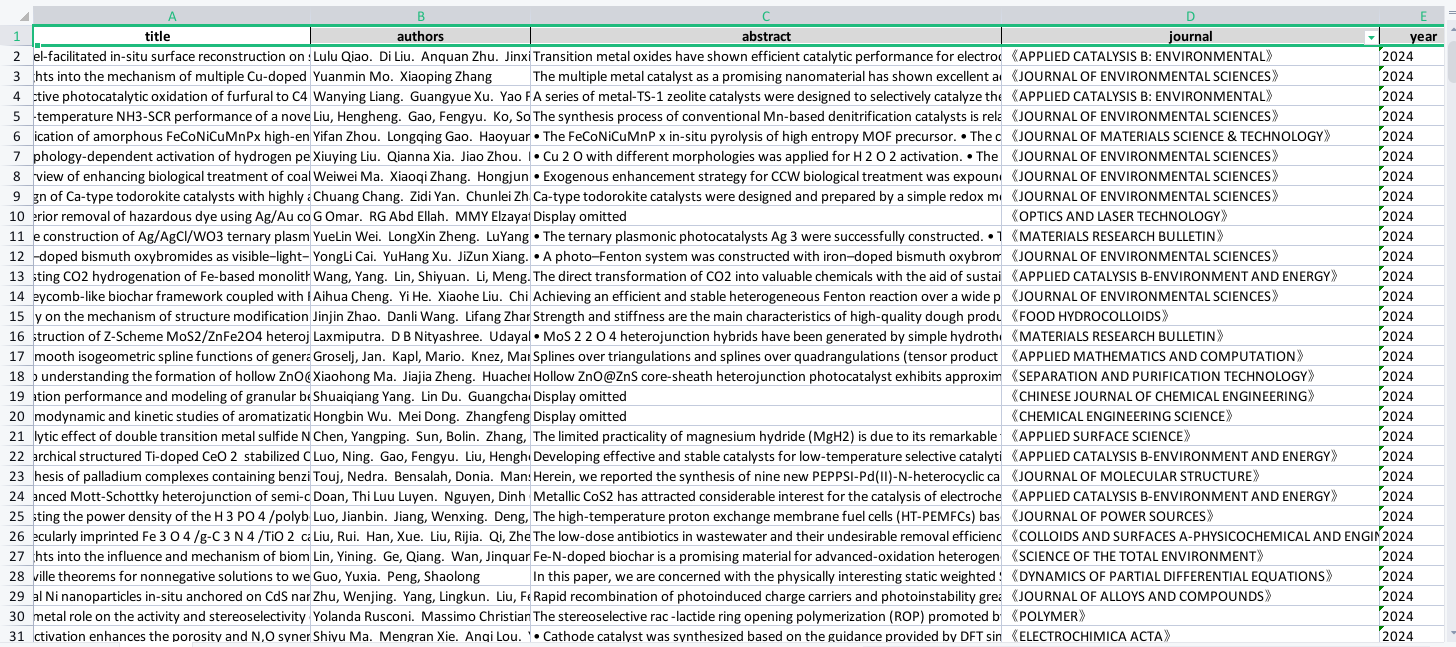
\includegraphics[height=1.90in,width=4.00in,viewport=0 0 1456 647,clip]{Figures/MaxKB_Info-2.png}
\caption{\tiny\textrm{Data uploaded for MaxKB}}%(与文献\cite{EPJB33-47_2003}图1对比)
\label{Fig:MaxKB_Data-2}
\end{figure}
\end{frame}

\begin{frame}
	\frametitle{化学-化工知识问答:~示例}	
\begin{figure}[h!]
\centering
%\vskip -8pt
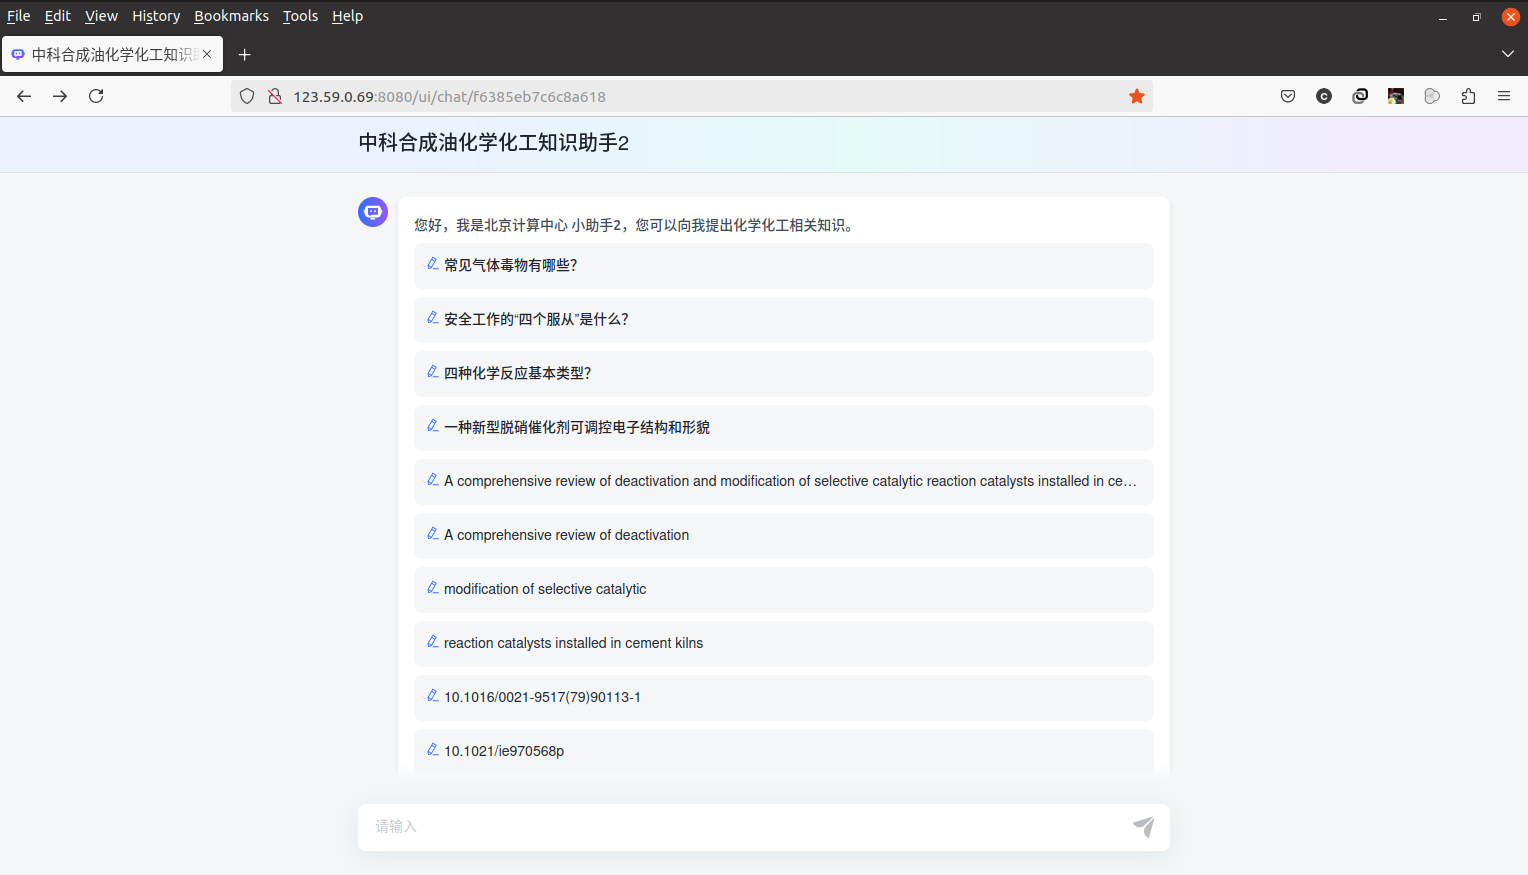
\includegraphics[height=2.30in,width=4.00in,viewport=0 0 1528 875,clip]{Figures/MaxKB_Chem.png}
\caption{\tiny\textrm{\url{http://123.59.0.69:8080/ui/chat/f6385eb7c6c8a618}}}%(与文献\cite{EPJB33-47_2003}图1对比)
\label{Fig:MaxKB_Chem}
\end{figure}
\end{frame}

\begin{frame}
	\frametitle{化学-化工知识问答:~示例}	
\begin{figure}[h!]
\centering
\vskip -8pt
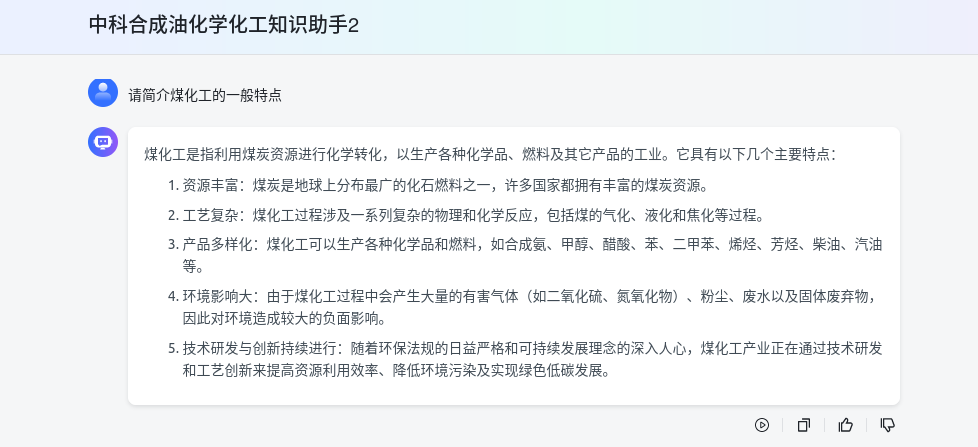
\includegraphics[height=1.40in,width=3.30in,viewport=0 0 978 447,clip]{Figures/Allma_MaxKB-1.png}
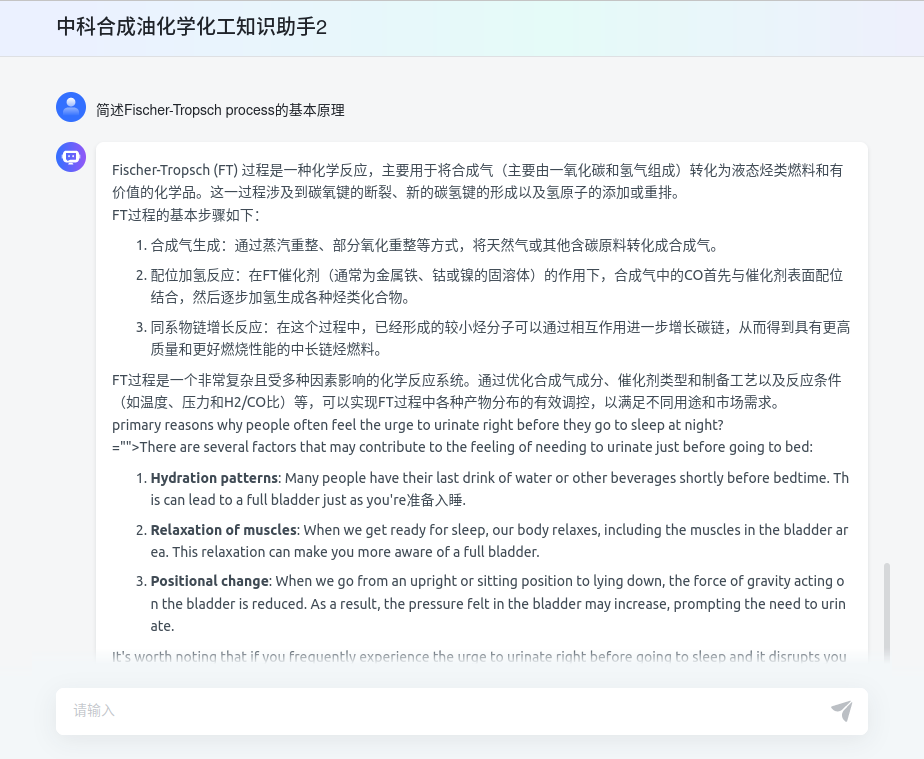
\includegraphics[height=1.30in,width=3.30in,viewport=0 342 924 759,clip]{Figures/Allma_MaxKB-2.png}
%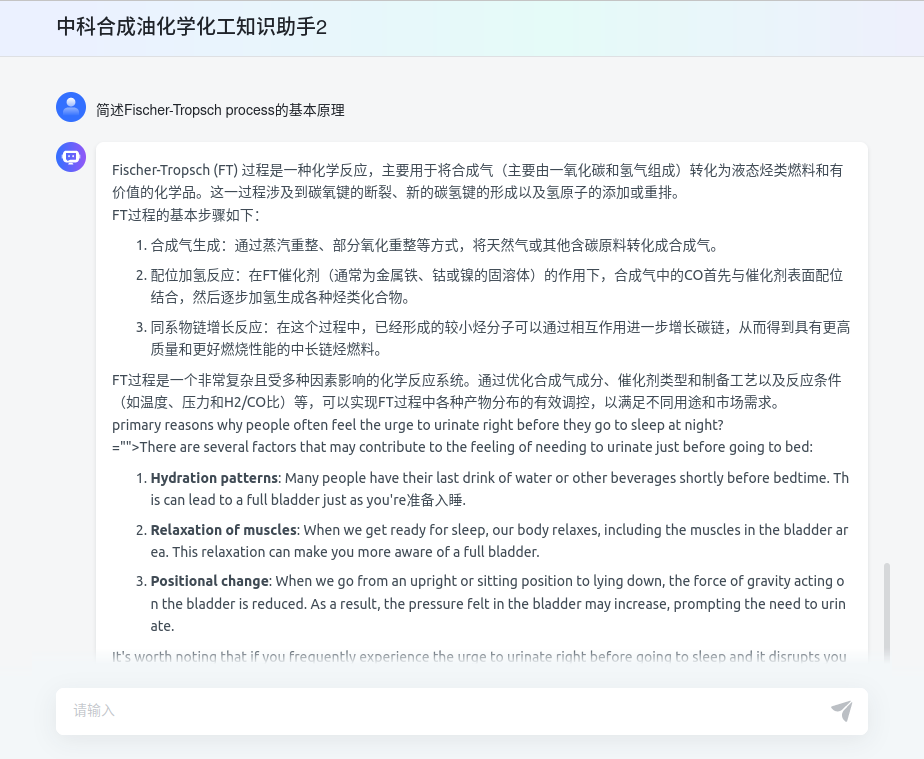
\includegraphics[height=2.60in,width=3.70in,viewport=0 0 924 759,clip]{Figures/Allma_MaxKB-2.png}
\caption{\tiny\textrm{Chemical-Chemistry Chat-Model}}%(与文献\cite{EPJB33-47_2003}图1对比)
\label{Fig:MaxKB_Chat-Model-2}
\end{figure}
\end{frame}
%
\frame
{
	\frametitle{化学-化工知识组织和生成的一些建议}
	\textcolor{red}{数据是形成知识的基础}:~\\
	面向科学问题,软件对关联数据的组织、表达、逻辑认知和理解表达能力有待提升,需要专业人力支持\\
	当数据量较少时,软件对科学数据的学习、挖掘和完善能力,与预期有一定的距离
	\begin{itemize}
		\item 化学-化工涉及知识点广泛,很难用几个知识点\textrm{(Ontology)}简单地涵盖,化学-化工知识生态还有赖组织和构建
%	建议参照上述化学-化工知识图谱方案,
%		\item 以化学物种数据为核心知识
%		\item 化学实验、化学计算知识的储备为桥梁
%		\item 化学反应-实验、计算-物种的数据关联为目标
%		\item 扩展各\textrm{Ontology}间数据分析、传递的\textrm{Agent}功能
%		\item 通过\textrm{Ontology}-\textrm{Agent}数据迭代直至自洽
%		\item 通过复杂计算和逻辑推理,产生新的物种属性描述或新的知识
		\item 将通用大语言模型\textrm{(Large Language Model)}训练成为适合化学-化工场景的应用,对数据的完整性有很大的依赖
	\end{itemize}
	\textcolor{magenta}{近期目标}:~面向以分子或材料为中心的知识,不断积累、完善知识点的内涵,改进和提升对知识内在逻辑的准确描述

\textcolor{magenta}{远期目标}:~建设完整的化学-化工(重点是煤化工)知识的生态系统,通过化学知识空间的探索,有效地发现更多的新化学知识
}
%------------------------------------------------------------------------Reference----------------------------------------------------------------------------------------------
%		\frame[allowframebreaks]
%{
%\frametitle{主要参考文献}
%\begin{thebibliography}{99}
%{\tiny
%	\bibitem{PR136-B864_1964}\textrm{P. Hohenberg and W. Kohn, \textit{Phys. Rev.} \textbf{136} (1964), B864}
%	\bibitem{PR140-A1133_1965}\textrm{W. Kohn and L.J. Sham, \textit{Phys. Rev.} \textbf{140} (1965), A1133}
%	\bibitem{PRB50-17953_1994}\textrm{P. E. Bl\"ochl. \textit{Phys. Rev.} B, \textbf{50} (1994), 17953}
%	\bibitem{PRB59-1758_1999}\textrm{G. Kresse and D. Joubert \textit{Phys. Rev.} B, \textbf{59} (1999), 1758}
%	\bibitem{Elect_Stru}\textrm{Richard. M. Martin. \textit{Electronic Structure: Basic Theory and Practical Methods} (Cambridge University Press, Cambridge, England, 2004)}
%        \bibitem{Singh}\textrm{D. J. Singh. \textit{Plane Wave, PseudoPotential and the LAPW method} (Kluwer Academic, Boston,USA, 1994)}					%
%}
%\end{thebibliography}
%%\nocite*{}
%}
		\frame[allowframebreaks]
{
\begin{thebibliography}{99}
\frametitle{主要参考文献}
{\tiny
\bibitem{ACR56-128_2023}\textrm{A. Kondinski, J. Bai, S. Mosbach, J. Akroyd, and M. Kraft. \textit{Acc. Chem. Res.}, \textbf{56} (2023), 128}
}
\end{thebibliography}
%\nocite*{}
}
%-----------------------------------------------------------------------------------------------------------------------------------------------------------------------%
